% !TeX encoding = UTF-8

% 载入 SJTUThesis 模版
\documentclass[type=master, openright]{sjtuthesis}
% 选项
%   type=[doctor|master|bachelor|course],     % 可选(默认:doctor),论文类型
%   zihao=[-4|5],                             % 可选(研究生默认:-4,本科默认:5),正文字号大小
%   language=[chinese|english],               % 可选(默认:chinese),论文的主要语言
%   review,                                   % 可选(默认:关闭),盲审模式
%   [twoside|oneside]                         % 可选(默认:twoside),单双页模式

% 论文基本配置,加载宏包等全局配置
% % !TEX root = ./main.tex

\sjtusetup{
  %
  %******************************
  % 注意:
  %   1. 配置里面不要出现空行
  %   2. 不需要的配置信息可以删除
  %******************************
  %
  % 信息录入
  %
  info = {%
    %
    % 标题
    %
    title           = {上海交通大学学位论文 \LaTeX{} 模板示例文档},
    title*          = {A Sample Document for \LaTeX-based SJTU Thesis Template},
    %
    % 标题页标题
    %   可使用“\\”命令手动控制换行
    %
    % display-title   = {上海交通大学学位论文\\ \LaTeX{} 模板示例文档},
    % display-title*  = {A Sample Document \\ for \LaTeX-based SJTU Thesis Template},
    %
    % 页眉标题
    %
    % running-title   = {示例文档},
    % running-title*  = {Sample Document},
    %
    % 关键词
    %
    keywords        = {上海交大, 饮水思源, 爱国荣校},
    keywords*       = {SJTU, master thesis, XeTeX/LaTeX template},
    %
    % 姓名
    %
    author          = {某\quad{}某},
    author*         = {Mo Mo},
    %
    % 指导教师
    %
    supervisor      = {某某教授},
    supervisor*     = {Prof. Mou Mou},
    %
    % 副指导教师
    %
    % assisupervisor  = {某某教授},
    % assisupervisor* = {Prof. Uom Uom},
    %
    % 学号
    %
    id              = {0010900990},
    %
    % 学位
    %   本科生不需要填写
    %
    degree          = {工学硕士},
    degree*         = {Master of Engineering},
    %
    % 专业
    %
    major           = {某某专业},
    major*          = {A Very Important Major},
    %
    % 所属院系
    %
    department      = {某某系},
    department*     = {Depart of XXX},
    %
    % 课程名称
    %   仅课程论文适用
    %
    course          = {某某课程},
    %
    % 答辩日期
    %   使用 ISO 格式 (yyyy-mm-dd);默认为当前时间
    %
    % date            = {2014-12-17},
    %
    % 资助基金
    %
    % fund  = {
    %           {国家 973 项目 (No. 2025CB000000)},
    %           {国家自然科学基金 (No. 81120250000)},
    %         },
    % fund* = {
    %           {National Basic Research Program of China (Grant No. 2025CB000000)},
    %           {National Natural Science Foundation of China (Grant No. 81120250000)},
    %         },
  },
  %
  % 风格设置
  %
  style = {%
    %
    % 本科论文页眉 logo 颜色 (red/blue/black)
    %
    % header-logo-color = black,
  },
  %
  % 名称设置
  %
  name = {
    % bib               = {References},
    % acknowledgements  = {谢\hspace{\ccwd}辞},
    % publications      = {攻读学位期间完成的论文},
  },
}

% 使用 BibLaTeX 处理参考文献
%   biblatex-gb7714-2015 常用选项
%     gbnamefmt=lowercase     姓名大小写由输入信息确定
%     gbpub=false             禁用出版信息缺失处理
\usepackage[backend=biber,style=gb7714-2015,gbpub=false]{biblatex}
% 文献表字体
% \renewcommand{\bibfont}{\zihao{-5}}
% 文献表条目间的间距
\setlength{\bibitemsep}{0pt}
% 导入参考文献数据库
\addbibresource{bibdata/thesis.bib}

% 定义图片文件目录与扩展名
\graphicspath{{figures/}}
\DeclareGraphicsExtensions{.pdf,.eps,.png,.jpg,.jpeg}

% 确定浮动对象的位置,可以使用 [H],强制将浮动对象放到这里(可能效果很差)
% \usepackage{float}

% 固定宽度的表格
% \usepackage{tabularx}

% 表格中支持跨行
\usepackage{multirow}

% 表格中数字按小数点对齐
\usepackage{dcolumn}
\newcolumntype{d}[1]{D{.}{.}{#1}}

% 使用长表格
\usepackage{longtable}

% 附带脚注的表格
\usepackage{threeparttable}

% 附带脚注的长表格
\usepackage{threeparttablex}

% 算法环境宏包
\usepackage[ruled,vlined,linesnumbered]{algorithm2e}
% \usepackage{algorithm, algorithmicx, algpseudocode}

% 代码环境宏包
\usepackage{listings}
\lstnewenvironment{codeblock}[1][]%
  {\lstset{style=lstStyleCode,#1}}{}

% 物理科学和技术中使用的数学符号,定义了 \qty 命令,与 siunitx 3.0 有冲突
% \usepackage{physics}

% 直立体数学符号
\newcommand{\dd}{\mathop{}\!\mathrm{d}}
\newcommand{\ee}{\mathrm{e}}
\newcommand{\ii}{\mathrm{i}}
\newcommand{\jj}{\mathrm{j}}

% 国际单位制宏包
\usepackage{siunitx}

% 定理环境宏包
\usepackage{ntheorem}
% \usepackage{amsthm}

% 绘图宏包
\usepackage{tikz}
\usetikzlibrary{shapes.geometric, arrows}

% 一些文档中用到的 logo
\usepackage{hologo}
\newcommand{\XeTeX}{\hologo{XeTeX}}
\newcommand{\BibLaTeX}{\textsc{Bib}\LaTeX}

% 借用 ltxdoc 里面的几个命令方便写文档
\DeclareRobustCommand\cs[1]{\texttt{\char`\\#1}}
\providecommand\pkg[1]{{\sffamily#1}}

% 自定义命令

% E-mail
\newcommand{\email}[1]{\href{mailto:#1}{\texttt{#1}}}

% hyperref 宏包在最后调用
\usepackage{hyperref}

% !TEX root = ./main.tex

\sjtusetup{
  %
  %******************************
  % 注意:
  %   1. 配置里面不要出现空行
  %   2. 不需要的配置信息可以删除
  %******************************
  %
  % 信息录入
  %
  info = {%
    %
    % 标题
    %
    title           = {蛋白质序列和药物分子序列的表征学习},
    title*          = {Representation learning of protein sequences and drug sequences},
    %
    % 标题页标题
    %   可使用“\\”命令手动控制换行
    %
    % display-title   = {上海交通大学学位论文\\ \LaTeX{} 模板示例文档},
    % display-title*  = {A Sample Document \\ for \LaTeX-based SJTU Thesis Template},
    %
    % 页眉标题
    %
    % running-title   = {示例文档},
    % running-title*  = {Sample Document},
    %
    % 关键词
    %
    keywords        = {上海交大, 饮水思源, 爱国荣校},
    keywords*       = {SJTU, master thesis, XeTeX/LaTeX template},
    %
    % 姓名
    %
    author          = {靳\quad{}远},
    author*         = {Yuan Jin},
    %
    % 指导教师
    %
    supervisor      = {杨旸副教授},
    supervisor*     = {Prof. Yang Yang},
    %
    % 副指导教师
    %
    % assisupervisor  = {某某教授},
    % assisupervisor* = {Prof. Uom Uom},
    %
    % 学号
    %
    id              = {119033910073},
    %
    % 学位
    %   本科生不需要填写
    %
    degree          = {工学硕士},
    degree*         = {Master of Engineering},
    %
    % 专业
    %
    major           = {计算机技术},
    major*          = {Computer technology},
    %
    % 所属院系
    %
    department      = {计算机科学与技术系},
    department*     = {Department of Computer Science and Technology},
    %
    % 课程名称
    %   仅课程论文适用
    %
    % course          = {某某课程},
    %
    % 答辩日期
    %   使用 ISO 格式 (yyyy-mm-dd);默认为当前时间
    %
    % date            = {2014-12-17},
    %
    % 资助基金
    %
    % fund  = {
    %           {国家 973 项目 (No. 2025CB000000)},
    %           {国家自然科学基金 (No. 81120250000)},
    %         },
    % fund* = {
    %           {National Basic Research Program of China (Grant No. 2025CB000000)},
    %           {National Natural Science Foundation of China (Grant No. 81120250000)},
    %         },
  },
  %
  % 风格设置
  %
  style = {%
    %
    % 本科论文页眉 logo 颜色 (red/blue/black)
    %
    % header-logo-color = black,
  },
  %
  % 名称设置
  %
  name = {
    % bib               = {References},
    % acknowledgements  = {谢\hspace{\ccwd}辞},
    % publications      = {攻读学位期间完成的论文},
  },
}

% 使用 BibLaTeX 处理参考文献
%   biblatex-gb7714-2015 常用选项
%     gbnamefmt=lowercase     姓名大小写由输入信息确定
%     gbpub=false             禁用出版信息缺失处理
\usepackage[backend=biber,style=gb7714-2015,gbpub=false]{biblatex}
% 文献表字体
% \renewcommand{\bibfont}{\zihao{-5}}
% 文献表条目间的间距
\setlength{\bibitemsep}{0pt}
% 导入参考文献数据库
\addbibresource{bibdata/thesis.bib}

% 定义图片文件目录与扩展名
\graphicspath{{figures/}}
\DeclareGraphicsExtensions{.pdf,.eps,.png,.jpg,.jpeg}

% 确定浮动对象的位置,可以使用 [H],强制将浮动对象放到这里(可能效果很差)
% \usepackage{float}

% 固定宽度的表格
% \usepackage{tabularx}

% 表格中支持跨行
\usepackage{multirow}

% 表格中数字按小数点对齐
\usepackage{dcolumn}
\newcolumntype{d}[1]{D{.}{.}{#1}}

% 使用长表格
\usepackage{longtable}

% 附带脚注的表格
\usepackage{threeparttable}

% 附带脚注的长表格
\usepackage{threeparttablex}

% 算法环境宏包
\usepackage[ruled,vlined,linesnumbered]{algorithm2e}
% \usepackage{algorithm, algorithmicx, algpseudocode}

% 代码环境宏包
\usepackage{listings}
\lstnewenvironment{codeblock}[1][]%
  {\lstset{style=lstStyleCode,#1}}{}

% 物理科学和技术中使用的数学符号,定义了 \qty 命令,与 siunitx 3.0 有冲突
% \usepackage{physics}

% 直立体数学符号
\newcommand{\dd}{\mathop{}\!\mathrm{d}}
\newcommand{\ee}{\mathrm{e}}
\newcommand{\ii}{\mathrm{i}}
\newcommand{\jj}{\mathrm{j}}

% 国际单位制宏包
\usepackage{siunitx}

% 定理环境宏包
\usepackage{ntheorem}
% \usepackage{amsthm}

% 绘图宏包
\usepackage{tikz}
\usetikzlibrary{shapes.geometric, arrows}

% 一些文档中用到的 logo
\usepackage{hologo}
\newcommand{\XeTeX}{\hologo{XeTeX}}
\newcommand{\BibLaTeX}{\textsc{Bib}\LaTeX}

% 借用 ltxdoc 里面的几个命令方便写文档
\DeclareRobustCommand\cs[1]{\texttt{\char`\\#1}}
\providecommand\pkg[1]{{\sffamily#1}}

% 自定义命令

% E-mail
\newcommand{\email}[1]{\href{mailto:#1}{\texttt{#1}}}

% hyperref 宏包在最后调用
\usepackage{hyperref}


\begin{document}

%TC:ignore

% 标题页
\maketitle

% 原创性声明及使用授权书
\copyrightpage
% 插入外置原创性声明及使用授权书
% \copyrightpage[scans/sample-copyright-old.pdf]

% 前置部分
\frontmatter

% 摘要
\input{contents/abstract}

% 目录
\tableofcontents
% 插图索引
\listoffigures*
% 表格索引
\listoftables*
% 算法索引
\listofalgorithms*

% 符号对照表
% \input{contents/nomenclature}

%TC:endignore

% 主体部分
\mainmatter

% 正文内容
% \input{contents/intro}
% !TEX root = ../main.tex

\chapter{简介}

这是 \sjtuthesis 的示例文档,基本上覆盖了模板中所有格式的设置。建议大家在使用模
板之前,除了阅读《\sjtuthesis\ 使用文档》,这个示例文档也最好能看一看。

\section{二级标题}

\subsection{三级标题}

\subsubsection{四级标题}

Lorem ipsum dolor sit amet, consectetur adipiscing elit, sed do eiusmod tempor
incididunt ut labore et dolore magna aliqua. Ut enim ad minim veniam, quis
nostrud exercitation ullamco laboris nisi ut aliquip ex ea commodo consequat.
Duis aute irure dolor in reprehenderit in voluptate velit esse cillum dolore eu
fugiat nulla pariatur. Excepteur sint occaecat cupidatat non proident, sunt in
culpa qui officia deserunt mollit anim id est laborum.

\section{脚注}

Lorem ipsum dolor sit amet, consectetur adipiscing elit, sed do eiusmod tempor
incididunt ut labore et dolore magna aliqua. \footnote{Ut enim ad minim veniam,
quis nostrud exercitation ullamco laboris nisi ut aliquip ex ea commodo
consequat. Duis aute irure dolor in reprehenderit in voluptate velit esse cillum
dolore eu fugiat nulla pariatur.}

\section{字体}


上海交通大学是我国历史最悠久的高等学府之一,是教育部直属、教育部与上海市共建的全
国重点大学,是国家“七五”、“八五”重点建设和“211 工程”、“985 工程”的首批建
设高校。经过 115 年的不懈努力,上海交通大学已经成为一所“综合性、研究型、国际化”
的国内一流、国际知名大学,并正在向世界一流大学稳步迈进。 

{\songti 十九世纪末,甲午战败,民族危难。中国近代著名实业家、教育家盛宣怀和一批
  有识之士秉持“自强首在储才,储才必先兴学”的信念,于 1896 年在上海创办了交通大
  学的前身——南洋公学。建校伊始,学校即坚持“求实学,务实业”的宗旨,以培养“第
  一等人才”为教育目标,精勤进取,笃行不倦,在二十世纪二三十年代已成为国内著名的
  高等学府,被誉为“东方MIT”。抗战时期,广大师生历尽艰难,移转租界,内迁重庆,
  坚持办学,不少学生投笔从戎,浴血沙场。解放前夕,广大师生积极投身民主革命,学校
  被誉为“民主堡垒”。}

{\heiti 新中国成立初期,为配合国家经济建设的需要,学校调整出相当一部分优势专业、
  师资设备,支持国内兄弟院校的发展。五十年代中期,学校又响应国家建设大西北的号
  召,根据国务院决定,部分迁往西安,分为交通大学上海部分和西安部分。1959 年 3月
  两部分同时被列为全国重点大学,7 月经国务院批准分别独立建制,交通大学上海部分启
  用“上海交通大学”校名。历经西迁、两地办学、独立办学等变迁,为构建新中国的高等
  教育体系,促进社会主义建设做出了重要贡献。六七十年代,学校先后归属国防科工委和
  六机部领导,积极投身国防人才培养和国防科研,为“两弹一星”和国防现代化做出了
  巨大贡献。}

{\kaishu 改革开放以来,学校以“敢为天下先”的精神,大胆推进改革:率先组成教授代
  表团访问美国,率先实行校内管理体制改革,率先接受海外友人巨资捐赠等,有力地推动
  了学校的教学科研改革。1984 年,邓小平同志亲切接见了学校领导和师生代表,对学校
  的各项改革给予了充分肯定。在国家和上海市的大力支持下,学校以“上水平、创一流”
  为目标,以学科建设为龙头,先后恢复和兴建了理科、管理学科、生命学科、法学和人文
  学科等。1999 年,上海农学院并入;2005 年,与上海第二医科大学强强合并。至此,学
  校完成了综合性大学的学科布局。近年来,通过国家“985 工程”和“211 工程”的建
  设,学校高层次人才日渐汇聚,科研实力快速提升,实现了向研究型大学的转变。与此同
  时,学校通过与美国密西根大学等世界一流大学的合作办学,实施国际化战略取得重要突
  破。1985 年开始闵行校区建设,历经 20 多年,已基本建设成设施完善,环境优美的现
  代化大学校园,并已完成了办学重心向闵行校区的转移。学校现有徐汇、闵行、法华、七
  宝和重庆南路(卢湾)5 个校区,总占地面积 4840 亩。通过一系列的改革和建设,学校
  的各项办学指标大幅度上升,实现了跨越式发展,整体实力显著增强,为建设世界一流大
  学奠定了坚实的基础。}

{\ifcsname fangsong\endcsname\fangsong\else[无 \cs{fangsong} 字体。]\fi 交通大学
  始终把人才培养作为办学的根本任务。一百多年来,学校为国家和社会培养了 20余万各
  类优秀人才,包括一批杰出的政治家、科学家、社会活动家、实业家、工程技术专家和医
  学专家,如江泽民、陆定一、丁关根、汪道涵、钱学森、吴文俊、徐光宪、张光斗、黄炎
  培、邵力子、李叔同、蔡锷、邹韬奋、陈敏章、王振义、陈竺等。在中国科学院、中国工
  程院院士中,有 200 余位交大校友;在国家 23 位“两弹一星”功臣中,有 6 位交大校
  友;在 18 位国家最高科学技术奖获得者中,有 3 位来自交大。交大创造了中国近现代
  发展史上的诸多“第一”:中国最早的内燃机、最早的电机、最早的中文打字机等;新中国
  第一艘万吨轮、第一艘核潜艇、第一艘气垫船、第一艘水翼艇、自主设计的第一代战斗
  机、第一枚运载火箭、第一颗人造卫星、第一例心脏二尖瓣分离术、第一例成功移植同种
  原位肝手术、第一例成功抢救大面积烧伤病人手术等,都凝聚着交大师生和校友的心血智
  慧。改革开放以来,一批年轻的校友已在世界各地、各行各业崭露头角。}

{\ifcsname lishu\endcsname\lishu\else[无 \cs{lishu} 字体。]\fi 截至 2011 年 12
  月 31 日,学校共有 24 个学院 / 直属系(另有继续教育学院、技术学院和国际教育学
  院),19 个直属单位,12 家附属医院,全日制本科生 16802 人、研究生24495 人(其
  中博士研究生 5059 人);有专任教师 2979 名,其中教授 835 名;中国科学院院士 15
  名,中国工程院院士 20 名,中组部“千人计划”49 名,“长江学者”95 名,国家杰出
  青年基金获得者 80 名,国家重点基础研究发展计划(973 计划)首席科学家 24名,国
  家重大科学研究计划首席科学家 9名,国家基金委创新研究群体 6 个,教育部创新团队
  17 个。}

{\ifcsname youyuan\endcsname\youyuan\else[无 \cs{youyuan} 字体。]\fi 学校现有本
  科专业 68 个,涵盖经济学、法学、文学、理学、工学、农学、医学、管理学和艺术等九
  个学科门类;拥有国家级教学及人才培养基地 7 个,国家级校外实践教育基地 5个,国
  家级实验教学示范中心 5 个,上海市实验教学示范中心 4 个;有国家级教学团队 8个,
  上海市教学团队 15 个;有国家级教学名师 7 人,上海市教学名师 35 人;有国家级精
  品课程 46 门,上海市精品课程 117 门;有国家级双语示范课程 7 门;2001、2005 和
  2009 年,作为第一完成单位,共获得国家级教学成果 37 项、上海市教学成果 157
  项。}

% !TEX root = ../main.tex

\chapter{蛋白质和药物分子序列表征学习研究现状}

生命科学研究进入后基因组时代以来,基因组学、蛋白质组学的高速发展使得蛋白质信息和药物化学的信息量膨胀极为迅速。在过去的几十年里,随着测序技术的发展,公共数据库中的蛋白质序列和药物分子序列的数量呈现爆炸式增长。目前在蛋白质方面已经建立了 Uniprot、Prosite、Protein Data Bank(PDB)等大型数据库用于各种蛋白质功能分析任务的研究,在药物分子方面也建立了如 ChEMBL、DrugBank、SuperTarget 等权威数据库用于各种药物再利用和药物生成等任务的研究。随着蛋白质组学和基因组学带来的数据量,研发过程中积累的知识量以及机器学习算法的快速变化,以数据驱动的机器学习和深度学习方法极大的提高了人类对蛋白质领域和药物化学领域的理解,激发了更多的研究人员投入到相关的研究中。目前,研究人员已经提出了多种针对蛋白质序列和药物分子序列的编码工具,下面主要从序列编码方法和基于编码的序列预测模型两方面对蛋白质序列和药物分子序列的研究现状进行介绍。

\section{蛋白质序列表征学习研究现状}

\subsection{蛋白质序列编码方法}
一个优秀的蛋白质序列编码方法是所有蛋白质功能分析任务,例如蛋白质分类、蛋白质亚细胞定位、蛋白质结构预测等功能分析任务的基础。针对蛋白质序列研究的关键在于如何对蛋白质序列进行编码,从而提取到序列中潜在的结构和领域知识特征。近年来,随着硬件的提升以及深度学习的不断发展,自然语言处理中的词嵌入技术替代了传统的手工特征提取方式,在序列表示学习方面取得了突破性的进展。由于蛋白质序列和 NLP 中的文本序列存在一定的相似性,传统文本中的编码方式也被广泛应用到了蛋白质序列中。

ProtVec \cite{asgari2015continuous} 是由 Ehsaneddin 和 Mohammad 等人于 2015 年提出。他们提出了一种针对蛋白质序列的无监督数据驱动分布式表示,可以应用于生物信息学中的广泛问题,例如蛋白质可视化、蛋白质家族分类、蛋白质结构预测、蛋白质域提取等。他们使用 Swiss-Prot 大型语料库(共有 546,790 条蛋白质序列)来训练蛋白质序列的分布式表示。接下来,他们将蛋白质序列分解为子序列(即具有生物意义的单词),利用 n-gram 建模 \footnote{n-gram 表示由 n 个氨基酸组成的具有生物意义的单词} 来训练序列的通用分布式表示。与传统的 n-gram 重叠窗口不同的是,他们将一条序列分解成长度为 n 个相邻氨基酸残基滑动窗口构成的分词列表,针对不同的序列切分起始位置,一条蛋白质序列可以划分为 n 种有序非重叠单词的集合,因此得到了 $546,790 \times 3 = 1,640,370$ 条 3-gram 组成的语料库。之后,他们通过 Word2Vec \cite{mikolov2013distributed} 中的 Skip-gram 神经网络基于语料库训练 n-gram 词嵌入表示,表征序列的理化特性。在训练词向量表示时,Skip-gram 试图最大化观察到的单词序列上下文的概率,即对于给定的单词训练序列,通过找到它们对应的 $n$ 维向量,最大化其平均对数概率函数,从而单词的含义由其上下文(即相邻单词)表征。该方法的优势在于词嵌入向量只需训练一次,然后可用于编码特定问题中的蛋白质序列,无需重新训练,大大节省了资源和时间的消耗。

SeqVec \cite{heinzinger2019modeling} 是由 Heinzinger 和 Elnaggar 等人于 2019 年提出的基于深度学习的双向 ELMo \cite{peters1802deep} 模型的蛋白质序列表征学习方法。与 ProtVec 的核心思想一致,他们通过对大型未标记序列数据学习隐式的生物理化特性代替传统的显示搜索。他们在 UniRef50 数据集上训练了双向语言模型 ELMo,其中每条蛋白质序列被视为一个句子,每个氨基酸被视为一个单词。ELMo 模型在未标记的语料库上进行训练,通过给定该句子中所有先前的单词,来预测句子中最有可能出现的下一个单词。通过学习句子的概率分布,模型可以自主学习到句法和语义概念。经过训练的向量词嵌入表示是上下文化的,即给定单词的嵌入取决于其上下文。这样做的好处是两个相同的单词可以有不同的词嵌入表示,这取决于它们周围的词是否不同。之后他们通过将其应用到两个级别的任务来评估嵌入的预测能力,分别是每个残基(单词级别)和每个蛋白质(句子级别)的任务。结果表明,这种将无标签的语料库词嵌入迁移到下游任务中的方式是有效的,可以捕获蛋白质序列的理化特性。

UniRef

TAPE 


\subsection{蛋白质序列分类模型}



\section{药物分子序列表征学习研究现状}

\subsection{药物分子序列编码方法}


\subsection{药物-靶标关系预测模型}





% !TEX root = ../main.tex

\chapter{词嵌入模型}

近些年,作为机器学习最重要的一个分支,深度学习成为科研人员关注的热点问题,并且深度学习模型在计算机视觉、自然语言处理、语音识别、数据挖掘等领域发挥了至关重要的作用。深度学习模型通过使机器模仿人类的感官和思想方式,挖掘大量的、多维度数据背后的潜在规则,解决了很多复杂的模式识别疑难问题,为人类迈向人工智能做出了突出贡献。不仅仅在上述领域,如今在生物信息学和基因组学方面,深度学习也带来了巨大的改变。在大数据时代,深度学习通过将生物医学大数据转化为有价值的领域知识极大简化了蛋白质功能研究和药物发现研究的历程。

传统的机器学习方法在研究的过程中,科研人员需要利用特征工程手动在原始序列数据的领域知识上提取特征,然后再部署相关的机器学习算法,这样的做法比较耗时而且极大的依赖于生物信息学和基因组学的专业知识。随着深度神经网络的兴起,传统的特征提取方法已经在很大程度上被序列编码方法,即词嵌入表征学习所取代。深度学习模型通过将组成生物序列的单词编码成稠密、连续的低维向量获得比离散特征提取表示更好的性能。由于在 NLP 领域的词向量和深度学习技术已经趋于成熟,同时生物序列和文本序列具有一定的相似性,可以通过将 NLP 中的词嵌入方法和深度学习模型迁移到生物信息学进行深入研究和探索。本章将重点介绍 NLP 领域中的词嵌入方法。

\section{基于神经网络的词嵌入方法}
词嵌入(Word Embedding)是一种将文本中的单词转化为稠密数字向量的方法。为了使计算机能够识别输入的特征,就需要把这些被转换成数字的向量以数字形式作为输入使用深度学习模型进行分析。

早期的词嵌入方法通常采用独热编码(One-hot)的方式,它使用一个词汇表大小的向量来表示文本中的词,其中只有对应于该词的项是1而所有其他的项都是零。One-hot 编码的最大问题在于不能表示词与词之间的相似性。我们通过点积计算向量之间的相似性。在One-hot编码中,语料库中任何两个词之间的点积总是为零,即任意两个词是正交的。随着深度学习的兴起,基于深度学习的词嵌入方法能够在没有任何人的干预下自主学习单词的潜在语义,同时可以表示词与词之间的相似性。我们不需要计算和存储关于某个庞大的数据集(可能是数十亿个句子)的全局信息,我们可以尝试创建一个模型,该模型将能够一次学习一个迭代,并最终能够根据上下文对单词的概率进行编码。其思想是设计一个以词向量为参数的模型。然后,针对特定的目标函数对模型进行训练。在每次迭代中,我们运行通过运行模型计算误差,并遵循相应的参数更新规则,该规则可以对导致误差的错误进行惩罚。通过这种机制,我们学习到了模型的词嵌入表征。目前,基于深度学习的词嵌入方法已经广泛应用于 NLP 领域的各种任务中,例如文本分类,情感分析,机器翻译等等。

蛋白质序列同自然语言处理中的文本一样,由很多单词排列组合构成。蛋白质序列由20几种连续的氨基酸构成,是研究蛋白质功能的基础。我们可以将组成蛋白质序列的氨基酸类比于组成文本的单词,将蛋白质序列信息类比于文本中句子的语义信息。因此,NLP 领域中的词嵌入方法非常适合于蛋白质序列领域的研究,下面将介绍4种本文用到的词嵌入方法。

\subsection{Word2Vec}
Word2Vec \cite{mikolov2013distributed} 词嵌入表征是由 Mikolov 等人于 2013 年提出的一种词嵌入方法。它包含两个学习模型,分别是 continuous bag-of-words (CBOW) 和 skip-gram. CBOW 旨在根据词向量从上下文信息中预测中心词,skip-gram则做了相反的事情,它从中心词预测上下文单词的分布(概率)。

\begin{figure}[!htp]
\centering
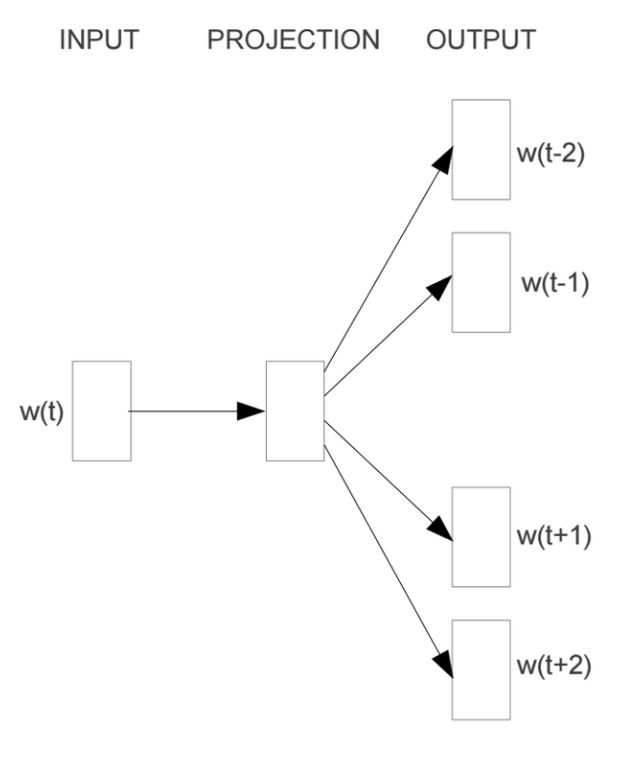
\includegraphics[width=0.6\textwidth]  {imgs/skip-gram.png} \\
\bicaption[Skip-gram\cite{mikolov2013distributed}图示]
    {Skip-gram\cite{mikolov2013distributed}图示。}
    {Model architecure of Skip-gram\cite{mikolov2013distributed}.}
\label{fig:skip-gram}
\end{figure}

这里我们以 skip-gram 模型为例详细的介绍。如图 \ref{fig:skip-gram} 所示,我们假设上下文的窗口为$2m$,即以中心词为中心,分别向左和向右选取$m$个单词,那么给定中心词预测上下文单词的概率为:

\begin{equation}
    P(\omega_c|\omega_o) = \frac{exp(u_o^{T} v_c)}{\sum_{i \in V} exp(u_i^{T} v_c)}
\tag{3-1}
\end{equation}
其中 $\omega_o$ 和 $\omega_c$ 分别代表中心词和上下文单词,$u_o$和$u_c$分别代表中心词向量和上下文词向量,$V$是全体词汇表。这个概率就是给定中心词的条件下,某个词是上下文词的概率。这里假设在给定中心词的条件下每个单词出现的概率是独立的,类似朴素贝叶斯的条件独立性假设,可以大大的简化运算,将上式改写为连乘的形式如下:

\begin{equation}
   \prod \limits_{t=1}^T \prod \limits_{-m\leq j \leq m, j \neq 0} P(\omega^{(t+j)}|\omega^{(t)})
\tag{3-2}
\end{equation}
其中$t$表示中心词的位置,$m$为窗口大小,这样就得到了每个中心词的计算上下文词的概率。在该公式中变量是上下文词向量和中心词向量,于是只要改变参数使得目标最大化就可以。这里使用极大似然估计,对上式取负对数得到:

\begin{equation}
   -\sum \limits_{t=1}^T \sum \limits_{-m\leq j \leq m, j \neq 0} log^{P(\omega^{(t+j)}|\omega^{(t)})}
\tag{3-3}
\end{equation}

对上式进行参数求导可以计算梯度,更新参数。梯度下降优化结束后,我们便能得到两个向量 $u$ 和 $v$,分别表示上下文词向量和中心词向量,这就是我们要找的词向量。

Word2Vec作为预训练的词嵌入方法,通常语料库包含上千万条数据,词汇表中的单词数量通常有上万个,因此在目标函数中计算所有单词的softmax概率需要消耗巨大的计算资源。对此,Mikolov等人提出了负采样和层级softmax方法简化模型的复杂度和参数量。

负采样的思想为,对于每个训练步骤,我们可以只采样几个反例而不是计算整个词汇表。层级 softmax 使用二叉树来表示词汇表中的所有单词。二叉树的每一个叶子节点都表示一个单词,从根节点到叶子节点都有一条独特的路径。一个单词作为输出词的概率表示为从根节点随机游走到该词叶节点的概率。计算成本从 $O(V)$ 降低为 $O(log^{V})$。

Daniel 和 David 等人 \cite{buchan2019inferring} 使用 Word2Vec 证明了蛋白质域在多域蛋白质的上下文中可能具有语义意义。在这项工作中,他们将多域蛋白质视为文本中的句子,其中域标识符视为句子中划分的单词。 通过使用 Interpro \cite{finn2017interpro} 真核蛋白质作为语料库,他们证明了 Word2Vec 可以获得具有功能意义的蛋白质域嵌入。


\subsection{GloVe}
Word2Vec 模型通过在上下文窗口中进行预测来学习单词嵌入,该模型具有捕获单词相似性的复杂语言模式的能力,但是未能利用全局共现统计。GloVe \cite{pennington2014glove} 是由 Pennington 等人于2014年提出的基于单词共现统计的词嵌入方法。相比之下,GloVe 由一个加权最小二乘模型组成,该模型在全局单词-单词间共现概率矩阵上进行训练,从而有效地利用了统计数据。 该模型生成了一个具有有意义子结构的词向量空间。它在单词类比任务上显示了最先进的性能,并且在几个单词相似性任务上优于其他的方法。

首先定义词与词之间的共现矩阵为 $X$,其中 $X_{ij}$ 是语料库中出现在单词 $i$ 上下文中单词 $j$ 的次数。定义 $X_i = \sum_{k} X_{ik}$ 表示单词 $i$ 的上下文所有单词的总个数。最终 $P_{ij} = P(j|i) = \frac{X_{ij}}{X_i}$ 表示单词 $j$ 出现在单词 $i$ 上下文的概率。

\begin{table}[!htbp]
\centering
\bicaption[GloVe \cite{pennington2014glove} 中共现矩阵示例]{GloVe \cite{pennington2014glove} 中共现矩阵示例。}{Example of GloVe \cite{pennington2014glove} co-occurrence matrix.}
\scalebox{1.25}{
\begin{tabular}{c|c|c|c|c}
\hline
概率和比率 & k=solid & k=gas & k=water & k=fashion\\
\hline
$P(k|ice)$ & $1.9\times10^{-4}$ & $6.6\times10^{-5}$ & $3.0\times10^{-3}$ & $1.7\times10^{-5}$\\
\hline
$P(k|stream)$ & $2.2\times10^{-5}$ & $7.8\times10^{-4}$ & $2.2\times10^{-3}$ & $1.8\times10^{-5}$\\
\hline
$P(k|ice)/p(k|stream)$ & 8.9 & $8.5\times10^{-2}$ & 1.36 & 0.96\\
\hline
\end{tabular}}
\label{tabel:glove-1}
\end{table}

表\ref{tabel:glove-1}表明,单词的词向量应该和单词共现概率的比率有关,而不是他们的概率本身。由表\ref{tabel:glove-1}看出 $P(i|k)/P(j|k)$ 的取值是有一定规律的,定义函数 $F(w_i,w_j,w_k) = P(i|k)/P(j|k)$, Pennington 等人对共现概率的比率进行了总结如表 \ref{table:glove-2} 所示:

\begin{table}[!htbp]
\centering
\bicaption[GloVe \cite{pennington2014glove} 中共现概率比率的规律。]{GloVe \cite{pennington2014glove} 中共现概率比率的规律。}{The law of GloVe \cite{pennington2014glove} co-occurrence probability ratio.}
\scalebox{1.2}{
\begin{tabular}{c|c|c}
\hline
$F(w_i,w_j,w_k)$ & 单词j,k相关 & 单词j,k不相关 \\
\hline
单词i,k相关 & 趋近于1 & 很大 \\
\hline
单词i,k不相关 & 很小 & 趋近于1\\
\hline
\end{tabular}}
\label{table:glove-2}
\end{table}

GloVe经过推理,定义目标函数(损失函数)如下:

\begin{equation}
  J = \sum \limits_{ik} f(X_{ik}){(w_i^{T}w_k + b_i + b_k - log(X_{ik}))}^2
\tag{3-4}
\end{equation}
其中$X_{ik}$表示单词$i$和$j$的共现次数,$f(X_{ik})$ 表示共现次数的权重因子,$f(x)$的定义如下:

\begin{equation}
 f(x) = \left\{
    \begin{array}{lr}
    (\dfrac{x}{x_{max}})^\alpha, & if x < x_{max} \\
    1, & otherwise\\
    \end{array}
\right.
\tag{3-5}
\end{equation}

函数$f(x)$有三个特点:(1)$f(0) = 0$,即两个单词没有共同出现过,权重为0;(2) $f(x)$是非减函数,如果两个单词共同出现的次数多,权重反而变小了,这违反了设置权重因子的初衷;(3)$f(x)$对于较大的$x$不能取太大的值,因为出现频率过高的词通常是一些无意义的单词。通过以上公式,可以将权重因子$f(x)$设置在一个合理的范围之内。根据经验,Pennington 等人任务 $x_{max} = 100, \alpha = \frac{3}{4}$ 是一个比较好的选择。 

综上所述,GloVe 模型通过对单词-单词共现矩阵中的非零元素进行训练来有效地利用全局统计信息,并生成具有有意义的子结构的向量空间。目前蛋白质的研究领域还没有使用 GloVe 词嵌入方法的研究成果。

\subsection{FastText}

FastText \cite{joulin2016bag} 是由 Facebook AI Research 开源的一个文本分类器,用于有效的学习单词嵌入表示和句子分类类别。模型拥有快捷的训练速度,适合在大型数据集上进行训练。相比于其他的文本分类模型,例如 SVM,逻辑回归,神经网络等,FastText 可以在保证分类准确率的情况下,大大的降低训练时间。


\begin{figure}[!htp]
\centering
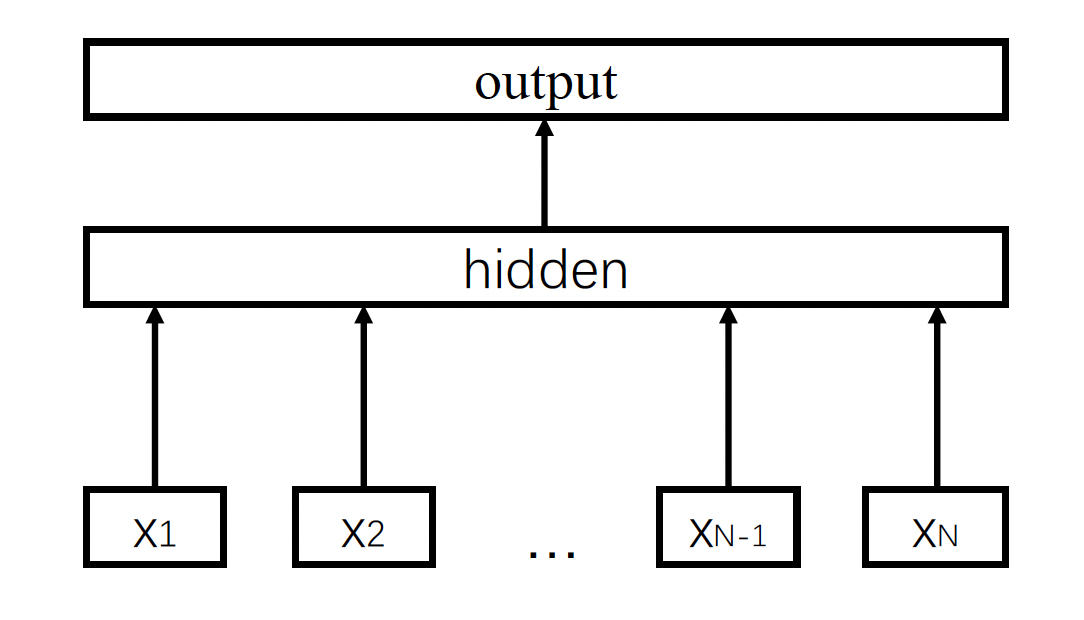
\includegraphics[width=0.9\textwidth]  {imgs/fasttext.png} \\
\bicaption[FastText \cite{joulin2016bag} 图示]
    {FastText \cite{joulin2016bag} 图示。}
    {Model architecure of FastText \cite{joulin2016bag}.}
\label{fig:fasttext}
\end{figure}

图\ref{fig:fasttext}为 FastText 的结构图。FastText 模型输入一个序列(可以是一句话,也可以是一段文本),输出这个序列在各个文本类别上的概率分布。FastText 模型结构和 Word2Vec 中的 CBOW 结构很相似,一共有三层,分别是输入层、隐藏层和输出层。首先将输入的序列划分为单词的特征向量,经过线性变换映射到隐藏层进行叠加求平均操作,最终线性变换映射到文本的类别标签。FastText 和 Word2Vec 的不同之处在于,在 Word2Vec 中将每一个单词视为要找到整个序列向量表示的最小单位;但在 FastText 中,采用 n-gram 对单词进行切分,即一个单词由 n-gram 个字符组成。为了加速训练的速度,FastText 中也采用了层级 softmax ,利用了类别分布不均衡的优势,通过使用哈夫曼编码建立基于类别表征的二叉树。因此,FastText 的核心工作是将构成序列的单词以及 n-gram 向量进行叠加平均操作得到序列向量,然后使用序列向量进行 softmax 多分类任务。

综上所述,FastText 使用一个浅层的神经网络能够达到媲美深度神经网络的分类精度,并且拥有高效的训练速度。可以在不使用 GPU 的情况下,利用 CPU 完成词嵌入向量的训练。Le 和 Huynh 等人\cite{le2019identifying} 结合 FastText 架构和氨基酸的嵌入表征来识别 SNARE。他们任务可以将 FastText 模型应用于生物信息学,可以为蛋白质测序预测提供基础。本文基于 FastText 模型结构构建了一个分类模型,可以同时用于蛋白质序列的嵌入表征学习以及蛋白质序列的分类任务。

\subsection{Doc2Vec}
Le 和 Mikolov 等人于 2014 年提出的 Doc2Vec 模型 \cite{le2014distributed} 是对 Word2Vec 模型的扩展。虽然 Word2Vec 可以提高比较准确的词向量,在一些任务中表现优异,但是还不存在一个有效的模型将它们结合成一个序列或者文档向量,因此 Doc2Vec 主要是对较大的文本块(例如段落或者整个文档等)的连续嵌入表示进行无监督学习。

和 Word2Vec 相似,Doc2Vec 也包含两个学习模型,一种是分布记忆的段落向量(PV-DM),类似于 Word2Vec 中的 CBOW 模型;另一种是分布词袋的段落向量(PV-DBOW),类似于 Word2Vec 中的 skip-gram 模型。
Doc2Vec 的训练过程和 Word2Vec 基本一致,每次迭代从一段话中利用滑动窗口采样固定长度的单词序列,其中的一个单词作为输出的预测词,其他单词作为输入词。不同之处在于,Doc2Vec 在 Word2Vec 的基础上增加了句子向量,同词向量一起作为输入层的输入,之后将所有的向量叠加求平均生成一个新的隐藏向量,进而使用这个隐藏向量预测滑动窗口内的预测词。句子向量在同一段文本的若干次滑动窗口迭代训练中是共享的,可以看作是该句子的主旨,因此拥有记忆功能,弥补了 Word2Vec 中忽略了本次窗口中训练的词以外文本中的其他词的不足。

Yang \cite{yang2018learned} 等人利用 Word2Vec 和 Doc2Vec 两种模型学习蛋白质的嵌入表征,由于蛋白质序列的长度相比普通的文本句子要长很多,因此 Doc2Vec 非常适合大文本的蛋白质序列嵌入表征学习。本文利用了 Doc2Vec 的 PV-DM 模型作为预训练任务学习蛋白质序列的嵌入表征。




% !TEX root = ../main.tex

\chapter{基于有监督预训练的蛋白质表征学习}

在过去的几十年里,蛋白质序列数据的快速增长为推断蛋白质的理化性质和功能提供了巨大的机会。 许多机器学习方法已成功应用于基于氨基酸序列信息的各种蛋白质分类任务,然而模型性能往往受到数据库中标记数据不足的影响。受到自然语言处理中预训练策略的启发,通过语言建模的无监督预训练已被引入生物序列分析从而缓解小数据问题。然而,这些无监督的预训练方法通常是计算密集型的,进行预训练需要消耗大量的计算资源,成本很高。

本章中,我们提出了一个用于进行蛋白质序列表征学习的预训练平台。研究的关键在于如何有效的利用蛋白质信息,尽可能地挖掘蛋白质中氨基酸表示的信息,通过预训练模型有效的处理氨基酸特征并对其进行表征学习。为了验证蛋白质序列的特征表示结果,我们开发的模型选取蛋白质研究中最典型的蛋白质分类问题对其进行研究,在三个蛋白质分类下游任务中(包括III 型分泌效应蛋白(T3SE)的识别、亚细胞定位的预测和信号肽的识别)进行实验。

本章将详细的介绍我们提出的 ProtPlat 模型,该模型完成了有监督的预训练氨基酸嵌入表征,进一步可以将预训练模型应用于各种蛋白质分类任务,同时我们实现了一个 Web 服务,用户可以下载经过预训练的词嵌入表征向量,并且通过提交自己的训练集和预测集获得蛋白质分类的预测类别。本章主要分为四个部分展开:分别是实验数据集构建、数据处理、基于蛋白质预训练表征学习的模型以及实验结果。

\section{实验数据集构建}
我们首先在 Pfam 数据库上对蛋白质序列进行大规模有监督的预训练表征学习,从而获得一个良好的氨基酸词嵌入表征。接着我们利用下游任务数据集对预训练的嵌入表征进行微调,使得他们在不同的下游任务上都有更好的表现。

\subsection{蛋白质表征学习预训练数据集} \label{4.1.1}
由于预训练需要大规模的语料库,因此我们使用 Pfam 数据库 \cite{finn2010pfam}。Pfam 是一个被广泛使用蛋白质家族结构域数据库,它是一系列蛋白质家族的集合,依赖多序列比对和隐马尔可夫模型(HMM)鉴定一个或者多个蛋白质的功能结构域,根据序列和结构的相似性将蛋白质序列划分为不同的家族,数据库中包括超过 3400 万个蛋白质序列。我们使用 Pfam 数据库中的 family 标签作为是预训练的目标,整个有监督预训练的过程是一个多分类问题。

由于 Pfam 数据中库蛋白质的 family 标签过多(2019 年发布的 32.0 版本中有 17929 个不同的 family 标签),为了避免数据分布极度不平衡导致的问题(如表 \ref{table:4.1.1}所示),我们去除了样本数小于500的蛋白质家族,总共得到了 7249 个蛋白质家族和 32853084 条蛋白质序列。

\begin{table}[!htbp]
\centering
\bicaption[Pfam 数据库中包含不同序列数的蛋白质家族数]{Pfam 数据库中包含不同序列数的蛋白质家族数。}{Numbers of protein families with different numbers of sequences in Pfam.}
\scalebox{1.3}{
\begin{tabular}{c|c}
\toprule
\# 蛋白质序列 & \# 蛋白质家族 \\
\midrule
$<$100 & 5474 \\ 
\hline
$<$200 & 7433 \\
\hline
$<$300 & 8775 \\
\hline
$<$500 & 10523 \\ 
\hline
$\geq$500 & 7249 \\
\bottomrule
\end{tabular}}
\label{table:4.1.1}
\end{table}


\subsection{下游蛋白质分类任务数据集}
为了评估经过预训练得到的词嵌入表征向量的性能,我们试验了三个下游蛋白质分类任务,如下所述。

\subsubsection{任务I:III 型分泌效应蛋白(T3SE)的识别}

III型分泌系统(TTSS)与许多革兰氏阴性病原体毒力因子的分泌有关。III 型分泌系统的效应蛋白(T3SE)直接从细菌细胞分泌到宿主细胞中,然后在疾病进展和免疫反应抑制中发挥作用。识别 III 型分泌效应蛋白有助于揭示 TTSS 的机制。然而,由于缺乏保留膜体或者分泌信号,T3SEs 的预测是一项特别具有挑战性的工作,现有方法主要是利用氨基酸序列的统计特征。这里,我们采用与 WEDeepT3 \cite{fu2019wedeept3} 相同的数据集 BEAN 2.0 \cite{dong2015bean},这是目前识别 T3SE 任务最大的数据集,其使用 CD-hit 工具 \cite{li2006cd} 去除蛋白质序列的冗余,并将序列一致性参数设置为 40\%。该数据集中一共包括 525 个训练样本(241 个 T3SE 和 284 个非 T3SE)和 138 个测试样本(46 个 T3SE 和 92 个非 T3SE)。 数据统计见表 \ref{table:4.1.2-1}。

\begin{table}[!htbp]
\centering
\bicaption[识别III型分泌效应蛋白数据集]{识别III型分泌效应蛋白数据集。}{Dataset of type III secreted effectors.}
\scalebox{1.3}{ 
\begin{tabular}{ c | c |c |c} 
 \toprule
  数据集 & T3SE & non-T3SE &总数\\  
 \midrule
 训练集 \#& 241 & 284 &525\\ 
 \hline
 测试集 \#& 46 & 92 &138\\ 
 \bottomrule
 \end{tabular}}
\label{table:4.1.2-1}
\end{table}

\subsubsection{任务II:预测蛋白质亚细胞定位}

蛋白质在细胞中的位置与其功能密切相关。只有在合适的亚细胞位置,蛋白质才能正确发挥其功能。细胞中蛋白质定位的计算预测一直是生物信息学领域的热门话题,目前大多数现有预测工具都是基于蛋白质序列和机器学习方法 \cite{cheng2018ploc, nair2005mimicking, 2010YLoc}。 我们使用经典的亚细胞定位基准集 BaCeILo \cite{pierleoni2006bacello},包括来自动物(Animals)、真菌(Fungi)和植物(Plants)的蛋白质序列,位于四个亚细胞区室,分别是细胞核、细胞质、线粒体和分泌途径。BaCeILo 的数据统计见表 \ref{table:4.1.2-2}。
% 此外,我们还使用了 DeepLoc[4]中使用的最新数据集,包括位于10个亚细胞区室的13858个蛋白质序列,分别是细胞核、细胞质、细胞外、线粒体、膜体、内质网、质体、高尔基体、溶酶体和过氧化物酶体。

\begin{table}[!htbp]
\centering
\bicaption[蛋白质亚细胞定位数据集]{蛋白质亚细胞定位数据集。}{Datasets of protein subcellular localization.}
\scalebox{1.3}{
 \begin{tabular}{ c | c | c | c | c | c} 
 \toprule
 数据集 & cy & mi & nu & sp & 总数 \\
 \midrule
 Animals 训练集 \# & 302 & 153 & 803 & 632 & 1890 \\ 
 \hline
 Animals 测试集 \#& 137 & 35 & 363 & 172 & 707 \\
 \hline
 Fungi 训练集 \#& 181 & 177 & 589 & 72 & 1019 \\
 \hline
 Fungi 测试集 \#& 30 & 11 & 122 & 16 & 179 \\
 \hline
 Plants 训练集 \#& 52 & 57 & 60 & 35 & 204 \\
 \hline
 Plants 测试集 \#& 6 & 10 & 61 & 6 & 83 \\
 \bottomrule
 \end{tabular}}
\begin{tablenotes}\scriptsize
\item [a] $^*$其中cy代表细胞核,mi代表细胞质,nu代表线粒体,sp代表分泌途径\\
\end{tablenotes}
 \label{table:4.1.2-2}
\end{table}

\subsubsection{任务III:信号肽的识别}
信号肽通常位于蛋白质序列末端,长度一般为 5 - 30 个氨基酸。信号肽的主要功能是促进蛋白质在细胞外分泌或定位于某些细胞器,因此信号肽的鉴定可以为揭示蛋白质功能提供线索。我们考虑了两种类型的信号肽,分别是由 SPase I (Sec/SPI) 切割的 Sec 底物和其他底物。我们使用 SignalP 5.0 \cite{armenteros2019signalp} 中提供的信号肽数据集,其中蛋白质来自真核生物(Archaea)、古细菌(Eukaryotes)、革兰氏阳性菌(Gram-positive)和革兰氏阴性菌(Gram-negative)。SignalP 5.0 数据集的数据统计见表 \ref{table:4.1.2-3}。

\begin{table}[!htbp]
\centering
\bicaption[信号肽的识别数据集]{信号肽的识别数据集。}{Datasets of signal peptides.}
\scalebox{1.3}{
 \begin{tabular}{c | c | c | c} 
 \toprule
 数据集 & Sec/SPI & 其他 & 总数 \\
 \midrule
 Archaea 训练集 \# & 10 & 45 & 55 \\ 
  \hline
 Archaea 测试集 \#& 50 & 132 & 182 \\
  \hline
 Eukaryotes 训练集 \#& 2404 & 7409 & 9813 \\
  \hline
 Eukaryotes 测试集 \#& 210 & 7247 & 7457 \\
  \hline
 Gram-negative 训练集 \#& 419 & 1126 & 1545 \\
  \hline
 Gram-negative 测试集 \#& 90 & 693 & 783 \\
  \hline
 Gram-positive 训练集 \#& 164 & 370 & 534 \\
  \hline
 Gram-negative 测试集 \#& 25 & 364 & 389 \\ 
 \bottomrule
 \end{tabular}}
 \label{table:4.1.2-3}
\end{table}


\section{数据处理}
\subsection{输入蛋白质序列的处理}
在蛋白质有监督的预训练任务和蛋白质分类任务中,输入的都是蛋白质序列。蛋白质序列是由20几种氨基酸排列组合形成的一串连续序列,因此在蛋白质序列中没有一个特定的划分边界,需要我们利用不同的序列切割方法进行词划分的尝试,然后利用深度学习网络在分词中提取特征表示信息。针对输入的蛋白质序列处理的关键首先在于对蛋白质序列进行切分,获取对应的词汇表。

和自然语言处理中的文本序列不同的是,蛋白质序列中没有已知的具有语义的单词作为划分边界,因此我们无法通过生物信息的意义判断合理的和不合理的分词。同时某个单词出现的频率和其表达的生物含义也无法意义对应。因此通常的做法是将蛋白质序列划分固定长度的短肽片段(即 k-mers,k 个氨基酸为一个单词)从而对词向量进行嵌入表征学习,应用到下游任务中。下面我们讨论了两种常用的蛋白质序列分割方法。

\subsubsection{不重叠的 $k-mer$ 切割方式}
在生物信息学领域,生物序列通常被分割成固定长度的 $k-mers$ 进行特征提取 \cite{asgari2015continuous, ofer2021language, yang2018learned, liu2019bioseq}。对于蛋白质序列来说,将连续的 $k$ 个氨基酸作为一个蛋白质的单词,接着对于剩余的蛋白质序列依次进行切分。通常,$k$ 的取值小于或等于 5,并且不能太大,因为随着 $k$ 的增加,$k-mer$ 词汇表空间将呈指数增长,这将导致极高的维度和单词频率的显著降低。最常见的不重叠 k-mer 切割方式是当 $k$ 的值为 1 时,此时每一个氨基酸表示一个单独的分词,此时蛋白质序列词汇表的大小为氨基酸的种类数。

不重叠的 $k-mer$ 切割方法的优点是简单方便。每个 $k-mer$ 不仅包含了单个氨基酸的信息,还包含其相邻 氨基酸的信息。但是,该分割方法的缺点也很明显。由于切分过于简单粗暴,直接将序列划分为 $k$ 个氨基酸组成的单词,导致将损失一部分的序列信息。另外,该切割方法只考虑固定长度的 $k-mer$ 分词。为了缓解这种限制,这里我们考虑包含所有长度小于或等于 k 的分词作为蛋白质序列的词汇表空间。以蛋白质序列 “MASPAAERKS” 为例,当k设置为3时,该序列的词汇表空间为
\{M, A, S, P, E, R, K, MA, SP, AA, ER, KS , MAS, PAA, ERK\} ,大小为 15。

\subsubsection{重叠的 $k-mer$ 切割方式}
使用不重叠 $k-mer$ 切割,切分起始位置的一点点偏移可能产生非常不同的切分词汇表。由于蛋白质序列的长度具有极大的不确定性,对于长度较短的蛋白质序列来说,对于切割起始位置的不同尤为敏感。为了避免这种由于单词划分带来的不确定性,重叠的 $k-mer$ 分割方法被广泛使用。该方法采用一个固定长度为 $k$ 的滑动窗口每次以步长为1的速度对蛋白质序列进行切割,在滑动窗口内的氨基酸作为一个蛋白质的单词,这样就考虑了序列中所有长度为 $k$ 的子串,比不重叠 $k-mer$ 的分割具有更大的特征空间。仍然以蛋白质序列 “MASPAAERKS” 为例,当k设置为3时,该序列的词汇表空间变为 \{M, A, S, P, E, R, K, MA, AS, SP, PA, AA, AE, ER, RK, KS, MAS, ASP, SPA, PAA, AAE, AER, ERK, RKS\},大小为24。可以看到, 重叠的 $k-mer$ 切割方式比不重叠的 $k-mer$ 切割方式可以保留更多的序列信息。和不重叠的 $k-mer$ 切割方式处理一样,我们考虑包含所有长度小于或等于 $k$ 的分词作为蛋白质序列的词汇表空间。

为了充分利用蛋白质序列的信息,我们接下来采用了重叠的 $k-mer$ 切割方式对蛋白质序列进行有监督的预训练,同时在蛋白质分类任务上进行验证。我们比较了使用这两种分割方法的模型性能,结果在第 4.4.1 节中讨论。

\subsection{预训练的数据处理}
在第 \ref{4.1.1} 节中提到,我们使用大型语料库 Pfam 数据库来执行有监督的预训练。Pfam 数据库的构建包括以下步骤(如图\ref{fig:data-process}所示):
\begin{itemize}
    \item [1)] 
    在 2019 年发布的 32.0 版本的 Pfam 数据库中下载了总共包含 17,772 个蛋白质家族和 34,353,433 条蛋白质序列; 
    \item [2)]
    提取每个蛋白质的家族(family)标签和蛋白质序列;
    \item [3)]
    通过删除少于 500 个样本的蛋白质家族,构建得到包含 7249 个蛋白质家族和 32,853,084 个序列的数据集。
  \end{itemize}

\begin{figure}[!htp] 
\centering
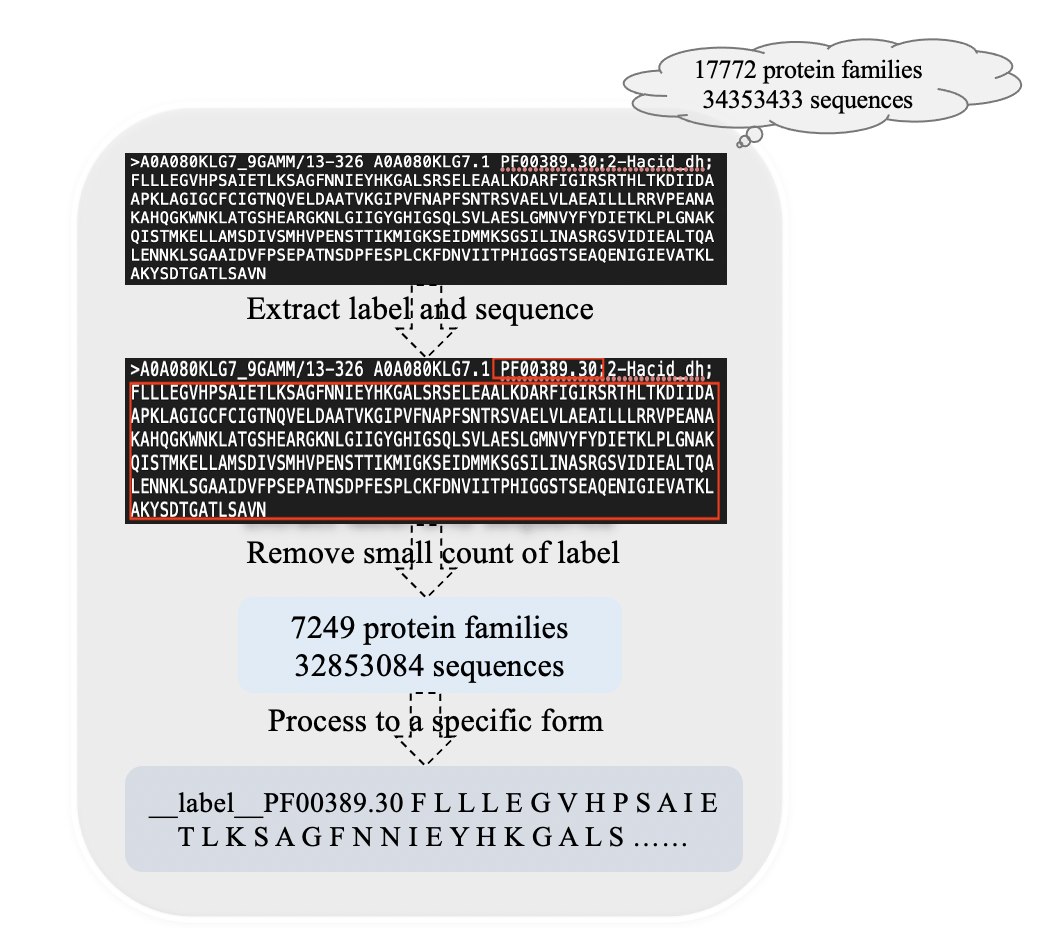
\includegraphics[width=0.95\textwidth]  {imgs/data-process.png}
\bicaption[Pfam 数据库的数据收集和过滤过程]
        {Pfam 数据库的数据收集和过滤过程。}
        {The data collection and filtering process of the Pfam database.}
\label{fig:data-process}
\end{figure}

\section{基于蛋白质预训练表征学习的模型}
\subsection{ProtPlat 模型}
为了描述 ProtPlat 模型的工作原理,我们定义了以下符号。

\begin{itemize}
    \item $C$:初始特征嵌入空间的大小,即用于分类任务的 k-mers (小于等于 k 的分词)的数量;
    \item $m$:嵌入表征向量的维度;
    \item $p$:隐藏层表征向量的维度;
    \item $n$:分类任务的标签数量;
    \item $V \in \mathbb{R}^{p*m}$:输入权重矩阵;
    \item $U \in \mathbb{R}^{n*p}$:输出权重矩阵
\end{itemize}

ProtPlat 模型的工作流程可以表述如下:
将 $(x^{(1)}, x^{(2)}, ..., x^{(C)}) \in \mathbb{R}^{m}$ 作为初始特征嵌入表征向量,通过一个全连接层获得嵌入表征向量,

\begin{equation}
    (h_1 = V \times x^{(1)}, h_2 = V \times x^{(2)},...,h_C = V \times x^{(C)}) \in \mathbb {R}^{p}.
\end{equation}

然后对所有的嵌入表征向量进行平均操作,得到平均嵌入表征向量,$\hat{h} \in \mathbb{R}^{p}$

\begin{equation}
    \hat{h} = \frac{\sum_{i\in \{1,2,\cdots, C\}} h_i}{C}. 
\end{equation}

接着将平均嵌入表征向量通过一个全连接层生成得分表示向量,$z \in \mathbb{R}^{n} $

\begin{equation}
    z = U \times \hat{h}.
\end{equation}

将得分表示向量通过层次 softmax 层转化为分类标签的概率分布,

\begin{equation}
    \hat{y} = softmax(z).
\end{equation}

ProtPlat 模型的主要结构是一个三层神经网络,如图 \ref{fig:protplat} 所示。模型的输入是一个 $C \times m$ 维矩阵,由蛋白质中长度小于或等于 $k$ 的分词的向量组成一个序列。例如,当 $k$ 设置为 3 时,输入涵盖所有的氨基酸、2-mer 和 3-mer 特征。其中每一个 $k-mer$ 的初始特征向量是它所包含的 $k$ 个氨基酸初始特征嵌入表示向量的平均值。

序列分类模型中的一个重要机制是层次 softmax 函数,它使用二叉树来表示所有类别。树中的每个叶子节点都表示一个类别,使得在具有大量标签的分类任务中有较高的学习效率。基于霍夫曼编码 \cite{han2015deep} 构建层次 softmax,对类别标签进行编码,可以大大减少模型的预测目标数量。模型中蛋白质序列的平均嵌入表示是一个隐藏变量,可以重复使用。这种架构类似于 CBow 模型 \cite{mikolov2013distributed},不同之处在于 ProtPlat 模型中的中心词被替换为序列标签。


\begin{figure}[!htp] 
\centering
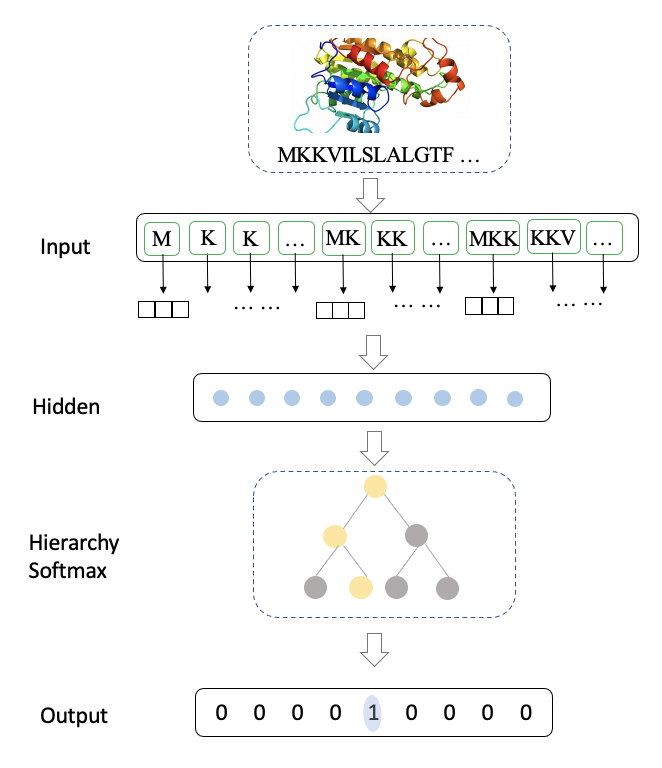
\includegraphics[width=0.85\textwidth]  {imgs/protplat.png}
\bicaption[ProtPlat 的模型架构]
        {ProtPlat 的模型架构。 $k-mer$ 嵌入表征向量送入神经网络并由隐藏层学习。输出类别标签由层次 Softmax 函数产生。}
        {Model architecture of ProtPlat. The k-mer embeddings are fed into the neural network and learned by the hidden layers. The output label is yielded by a hierarchy Softmax function. }
\label{fig:protplat}
\end{figure}

\subsection{两阶段训练过程}
为了将 ProtPlat 应用于下游任务,我们执行了一个两阶段的训练过程。

i) 预训练

我们使用 Pfam 数据库中的蛋白质序列和家族标签进行有监督的预训练,训练 ProtPlat 模型。 单个氨基酸的输入初始特征嵌入表示向量是随机初始化的,$k-mer$ 的初始特征嵌入表示向量是它所包含的 $k$ 个氨基酸初始特征嵌入表示向量的平均值。模型的输出是 Pfam 数据库中蛋白质序列所属的蛋白质家族标签。训练后,我们将每个氨基酸的嵌入表征向量保存为其经过预训练的特征嵌入表示向量,用于作为下游任务的输入初始特征嵌入表示向量(即 $x^{(i)}$)。

ii) 微调

微调阶段的训练过程与预训练几乎相同。不同之处在于输入和输出,其中氨基酸的输入是经过预训练的特征嵌入表示向量,$k-mer$ 的输入是它所包含的 $k$ 个氨基酸的经过预训练的特征嵌入表示向量的平均值,输出为下游分类任务的标签。

\section{实验结果}
\subsection{实验设置及评估指标}
对于预训练和微调过程,我们均随机抽取 20\% 的训练数据形成验证集。我们根据验证集上的模型性能选择最佳的超参数。表 \ref{table:4.4.1} 显示了 ProtPlat 中预训练阶段的超参数设置。值得注意的是,$k$ 的值是在预训练阶段确定的,在下游任务中保持不变。 对于每个下游任务,我们在其验证集上调整 epoch 和 learning rate。

\begin{table}[!htbp]
\centering
\bicaption[ProtPlat 中预训练阶段的超参数设置]{ProtPlat 中预训练阶段的超参数设置。}{Hyperparameter settings for pre-training in ProtPlat.}
\scalebox{1.3}{
\begin{tabular}{c|c}
\toprule
超参数 & 对应的值 \\
\midrule
k & 3 \\ 
\hline
epoch & 70 \\
\hline
learning rate & 0.15 \\
\hline
嵌入表征向量的维度 & 100 \\ 
\hline
隐藏层表征向量的维度 & 100 \\
\bottomrule
\end{tabular}}
\label{table:4.4.1}
\end{table}

为了评估 ProtPlat 模型的性能,我们在二元分类下游任务中使用了四个评估指标,包括准确率 (ACC)、$F_1$ 值 (F1 score)、presion (Pre) 和 recall (Rec)。它们的计算公式如公式(\ref{Eq:4-5})- 公式(\ref{Eq:4-8}) 所示。

\begin{equation}
    ACC = \frac{TP + TN}{TP + TN + FP + FN}
\label{Eq:4-5}
\end{equation}

\begin{equation}
    F_1 = \frac{2 * TP}{2 * TP + FP + FN}
\label{Eq:4-6}
\end{equation}

\begin{equation}
    Pre = \frac{TP}{TP + FP}
\label{Eq:4-7}
\end{equation}

\begin{equation}
    Rec = \frac{TP}{TP + FN}
\label{Eq:4-8}
\end{equation}
其中 $TP$、$TN$、$FP$ 和 $FN$ 分别表示真阳性、真阴性、假阳性和假阴性的数量。 

对于多分类问题,$F_1$ 值定义如公式(\ref{Eq:4-9})— 公式(\ref{Eq:4-11})所示:

\begin{equation}
    Pre = \frac{\sum TP_i}{\sum TP_i + \sum FP_i}
\label{Eq:4-9}
\end{equation}

\begin{equation}
    Rec = \frac{\sum TP_i}{\sum TP_i + \sum FN_i}
\label{Eq:4-10}
\end{equation}

\begin{equation}
    F_1 = \frac{2 * Pre * Rec}{Pre + Rec}
\label{Eq:4-11}
\end{equation}
其中,$i$ 代表多分类问题的类别索引,$TP_i$、$FP_i$ 和 $FN_i$ 分别表示第 i 个类别真阳性、假阳性和假阴性的数量。


\subsection{预训练表征学习的结果}
在这里,我们比较了经过预训练和没有经过预训练的 ProtPlat 模型的结果。经过预训练的 ProtPlat 模型使用预训练的嵌入表征向量作为每一个氨基酸的初始输入特征表示,而没有经过预训练的 ProtPlat 模型使用 one-hot 编码向量作为初始输入并随机初始化输入权重。

我们比较了它们在八个下游任务数据集上的性能,包括 T3SE 数据集、三个亚细胞定位数据集(来自 BaCeILo \cite{pierleoni2006bacello} 的植物、真菌和动物数据集)和四个信号肽数据集(来自 SignalP 5.0 \cite{armenteros2019signalp} 的古细菌、真核生物、革兰氏阳性和革兰氏阴性数据集)。结果如图 \ref{fig:pre-unpre} 所示。可以看出,预训练过程可以提高所有这些数据集的预测精度。$F_1$ 值增加了 0.03 — 0.08。此外,我们对性能差异进行了统计显着性分析。对于下游任务的每个数据集,我们分别在预训练和没有经过预训练的情况下运行 ProtPlat 模型 30 次,成对 $t$ 检验的 $p-value$ 值展示在表 \ref{table:4.4.2-1} 和 表 \ref{table:4.4.2-2} 中。对于所有的下游任务而言,$p-values$ 值都远小于 0.01,表明经过预训练的 ProtPlat 模型明显优于没有预训练的模型。

\begin{figure}[!htp] 
\centering
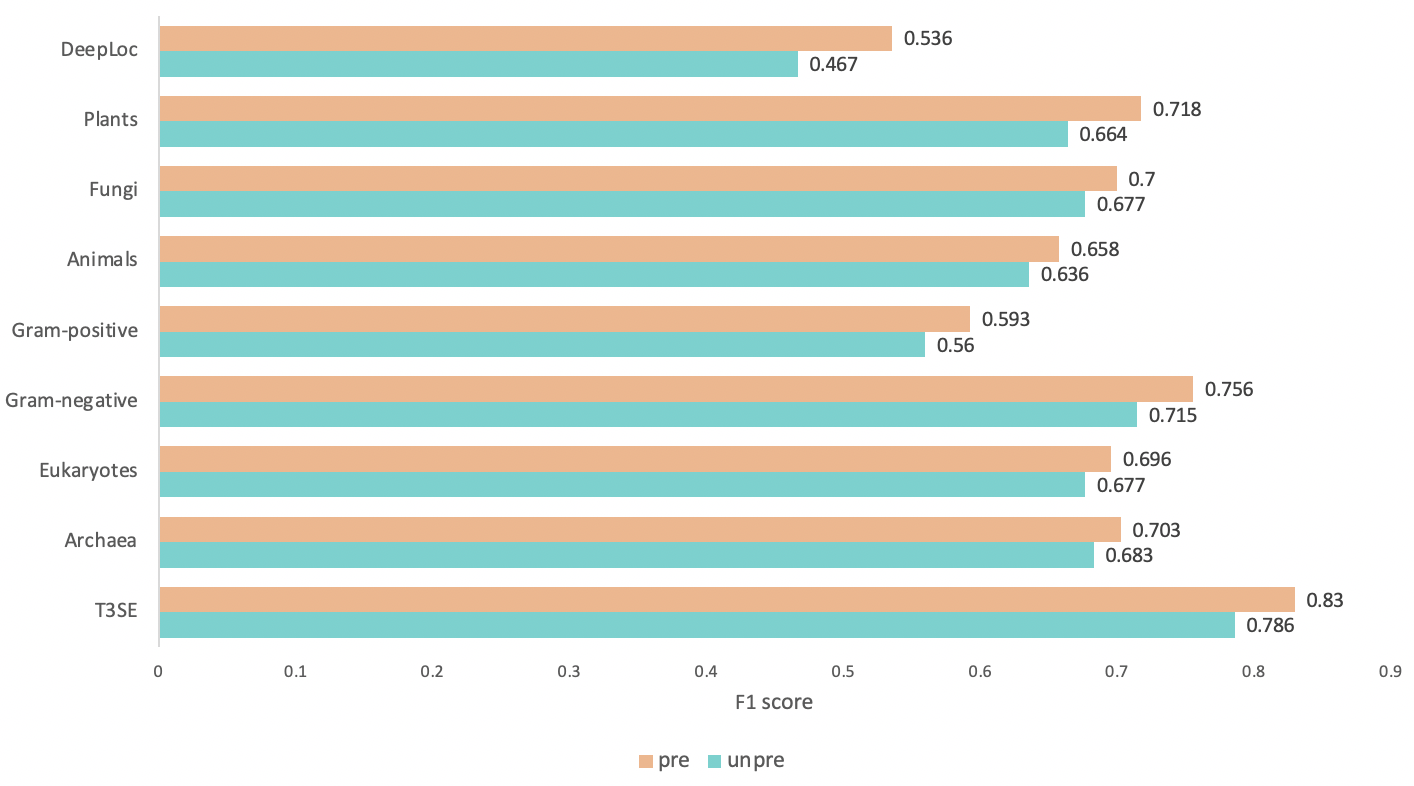
\includegraphics[width=1\textwidth]  {imgs/pre-unpre.png}
\bicaption[ProtPlat 有无经过预训练的 $F_1$ 值对比]
        {ProtPlat 有无经过预训练的 $F_1$ 值对比。}
        {F1 score comparison between models with and without pre-training. }
\label{fig:pre-unpre}
\end{figure}


\begin{table}[!htbp]
\centering
\bicaption[经过(w)和不经过(w/o)预训练的 Protplat 模型 ACC 的显着性分析]{经过(w)和不经过(w/o)预训练的 Protplat 模型 ACC 的显着性分析。}{Significance analysis of accuracy for models with (w) and without (w/o) pre-training.}
\begin{tabular}{c|c|c|c|c|c}
\toprule
\multirow{2}*{数据集} & \multicolumn{2}{c|}{平均值} & \multicolumn{2}{c|}{方差} & \multirow{2}*{p-value} \\
\cline{2-5}
&$w/o\quad pre$&$w\quad pre$&$w/o\quad pre$&$w\quad pre$ &   \\
\midrule
T3SE&0.786&0.830& 4.29E-05&3.34E-05& 6.39E-12\\
\hline
Animals&0.636&0.658&0.05E-05&1.68E-05 & 1.07E-08\\ 
\hline
Fungi&0.677&0.700& 3.41E-05&6.37E-05 &9.53E-07\\
\hline
Plants&0.664&0.718&3.79E-05&5.47E-05 &8.25E-13\\
\hline
Archaea&0.765&0.790& 5.13E-05&3.24E-05& 3.65E-07\\
\hline
Eukaryotes&0.923&0.947&3.21E-05&1.58E-05& 9.13E-09\\
\hline
Gram-negative&0.715&0.751&4.97E-05&8.62E-06&3.69E-10\\
\hline
Gram-positive&0.784&0.810& 3.47E-05&6.53E-05& 3.68E-09\\
\bottomrule
\end{tabular}
\label{table:4.4.2-1}
\end{table}

\begin{table}[!htbp]
\centering
\bicaption[经过(w)和不经过(w/o)预训练的 Protplat 模型 $F_1$ 值的显着性分析]{经过(w)和不经过(w/o)预训练的 Protplat 模型 $F_1$ 值的显着性分析。}{Significance analysis of F1 score for models with (w) and without (w/o) pre-training.}
\begin{tabular}{c|c|c|c|c|c}
\toprule
\multirow{2}*{数据集} & \multicolumn{2}{c|}{平均值} & \multicolumn{2}{c|}{方差} & \multirow{2}*{p-value} \\
\cline{2-5}
&$w/o\quad pre$&$w\quad pre$&$w/o\quad pre$&$w\quad pre$ &   \\
\midrule
T3SE&0.786&0.830& 4.29E-05&3.34E-05& 6.39E-12\\
\hline
Animals&0.636&0.658&0.05E-05&1.68E-05 & 1.07E-08\\ 
\hline
Fungi&0.677&0.700& 3.41E-05&6.37E-05 &9.53E-07\\
\hline
Plants&0.664&0.718&3.79E-05&5.47E-05 &8.25E-13\\
\hline
Archaea&0.683&0.703& 8.47E-05&4.27E-05& 2.56E-05\\
\hline
Eukaryotes&0.677&0.696&1.71E-05&2.01E-05& 1.68E-08\\
\hline
Gram-negative&0.715&0.756&1.39E-05&2.42E-05&4.50E-14\\
\hline
Gram-positive&0.56&0.593& 4.31E-05&5.32E-05& 3.61E-09\\
\bottomrule
\end{tabular}
\label{table:4.4.2-2}
\end{table}

\subsection{ProtPlat 与现有方法在下游任务上的比较}
\subsubsection{任务I:III 型分泌效应蛋白(T3SE)的识别}

III 型分泌效应子的识别是一个二元分类问题,即 T3SE 和非 T3SE。 为了评估 ProtPlat 模型的性能,我们将其与现有的代表性方法进行比较,包括 WEDeepT3 \cite{fu2019wedeept3}、BPBAac \cite{wang2011high}、EffectiveT3 \cite{arnold2009sequence}、T3\_MM \cite{wang2013t3_mm}、DeepT3 \cite{xue2019deept3}、Bastion3 \cite{wang2019bastion3} 和 BEAN 2.0 \cite{dong2015bean}。 

ProtPlat 模型在 WEDeepT3 的测试集上得到的结果如表\ref{table:4.4.3-1}所示。可以看出,ProtPlat取得了最好的性能。 与第二好的模型 WEDeepT3 相比,经过预训练的 ProtPlat 模型的 $F_1$ 值提高了 0.128,准确率提高了 0.021,这印证了预训练嵌入表征学习的分类性能。

\begin{table}[!htbp]
\centering
\bicaption[预测 III 型分泌效应蛋白的模型性能比较]{预测 III 型分泌效应蛋白的模型性能比较。}{Performance comparison for the prediction of type III secreted effectors.}
\scalebox{1.2}{
 \begin{tabular}{c | c | c } 
    \toprule
模型 & ACC & $F_1$ \\
 \midrule
WEDeepT3 & 0.812 & 0.705 \\ 
 \hline
BPBAac &0.609 &0.339\\
 \hline
EffectiveT3 &0.696 &0.512\\
 \hline
T3\_MM & 0.718 &0.581\\
 \hline
DeepT3 &0.594 &0.486\\
 \hline
Bastion3 &0.739 &0.673\\
 \hline
BEAN 2.0&0.761 &0.692\\
 \hline
ProtPlat & \textbf{0.833} & \textbf{0.833} \\ 
 \bottomrule
 \end{tabular}}
 \label{table:4.4.3-1}
\end{table}
其中,基线方法的准确率和 $F_1$ 值是从 WEDeepT3 \cite{fu2019wedeept3} 中提取的。所有方法都在相同的测试集上进行评估。


\subsubsection{任务II:预测蛋白质亚细胞定位}
对于蛋白质亚细胞定位,我们使用 BaCeILo \cite{pierleoni2006bacello} 中的数据集,并且与 Euk-mPLoc \cite{cheng2018ploc}、LOCTree \cite{nair2005mimicking}、BaCeILo \cite{pierleoni2006bacello}、 YLoc \cite{2010YLoc} 等基线方法进行比较。通过准确率(ACC)和 $F_1$ 值来评估模型的分类预测性能。对于所有的三个数据集植物(Plants)、真菌(Fungi)和动物(Animals),ProtPlat 都实现了具有竞争力的模型性能。尤其是在真菌(Fungi)数据集上,ProtPlat 明显优于其他模型($F_1$ 值和准确率(ACC)都提高了 10\% 以上),如表\ref{table:4.4.3-2}所示,这表明小数据集可能会从预训练中受益更多。对于小数据集本身来说标签数据量较少,提供的蛋白质领域信息较少,通过大数据量的预训练嵌入表征学习,可以为小数据集提供较为丰富的先验知识,解决了小数据集上蛋白质预测性能较低的问题。

基线模型的训练集不同 \cite{2010YLoc},并且很多基线模型都是更通用的预测器,可以预测 4 个以上的亚细胞位置,比如 YLoc-HighRes、YLoc+、MultiLoc2-HighRes、WoLF PSORT、Euk- mPLoc 和 LOCTree,因此它们的性能可能比专门为这四个位置训练的预测器差。值得注意的是,几乎所有的基线方法都利用了多个来源的信息作为输入特征,包括某些领域知识,例如蛋白质功能域和基因本体。相比之下,ProtPlat 使用 Pfam 数据库中的序列信息和蛋白质家族标签,这些信息是蛋白质一维表示信息,而不是针对于特定预测任务的特征,还可以获得与基线方法相当甚至更好的结果。对比结果表明,经过预训练嵌入表示的 ProtPlat 模型具有强大的学习能力,这在领域知识匮乏的情况下非常有用。

\begin{table}[!htbp]
\centering
\bicaption[预测蛋白质亚细胞定位的模型性能比较]{预测蛋白质亚细胞定位的模型性能比较。}{Performance comparison for protein subcellular location prediction.}
\scalebox{1.2}{
 \begin{tabular}{c|c|c|c|c|c|c} 
 \toprule
\multirow{2}*{模型}& \multicolumn{2}{c|}{Animals} & \multicolumn{2}{c|}{Fungi} & \multicolumn{2}{c}{Plants}\\
\cline{2-7}
& ACC & $F_1$ & ACC & $F_1$ & ACC & $F_1$  \\
\midrule
Euk-mPLoc & 0.61 & 0.54 & 0.60 & 0.56 & 0.46 & 0.37\\
 \hline
WoLF PSORT & 0.70 & 0.67 & 0.50 & 0.51 & 0.57 & 0.46 \\
 \hline
LOCTree & 0.62 & 0.58 & 0.47 & 0.43 & 0.70 & 0.58 \\
 \hline
BaCeILo & 0.64 & 0.66 & 0.57 & 0.60 & 0.69 & 0.56 \\
 \hline
MultiLoc2-HighRes & 0.68 & 0.71 & 0.53 & 0.58 & 0.62 & 0.54 \\
 \hline
MultiLoc2-LowRes & 0.73 & \textbf{0.76} & 0.60 & 0.61 & 0.76 & 0.64 \\
 \hline
YLoc+ & 0.58 & 0.67 & 0.48 & 0.51 & 0.58 & 0.49 \\
 \hline
YLoc-HighRes & 0.74 & 0.69 & 0.56 & 0.51 & 0.58 & 0.54 \\
 \hline
YLoc-LowRes &  \textbf{0.79} & 0.75 & 0.56 & 0.61 & 0.71 & 0.58 \\
 \hline
ProtPlat & 0.66 & 0.66 & \textbf{0.71} & \textbf{0.71} & \textbf{0.72} & \textbf{0.72}\\
 \bottomrule
 \end{tabular}}
 \label{table:4.4.3-2}
\end{table}
其中,基线方法的准确率(ACC)和 $F_1$ 值是从 YLoc \cite{2010YLoc} 中提取的。


\subsubsection{任务III:信号肽的识别}

对于信号肽的识别,我们执行二元分类任务并将 ProtPlat 与 SignalP 5.0 \cite{armenteros2019signalp} 中提到的 16 种基线方法进行比较。通过精度(Precision)、召回率(Recall)和 $F_1$ 值对模型预测性能进行评估。模型预测性能的结果如表 \ref{table:4.4.3-3} 所示。对于古细菌(Archaea)和革兰氏阴性(Gram-negative)数据集,ProtPlat 的 $F_1$ 值最高。总的来说,ProtPlat 的性能与 SignalP 5.0 相当,并且高于所有其他 15 个基线,其中SignalP 5.0 使用手工制作的特征和特定的架构来识别信号肽。对于真核生物(Eukaryotes
)数据集,ProtPlat 的精度和召回值更接近 SignalP 5.0,并且高于其他基线。对于 Gram-negative 数据集,ProtPlat 的结果接近 SignalP 5.0 的结果,精度值明显高于其他基线,召回值也更高。对于革兰氏阳性(Gram-positive)数据集,ProtPlat 实现了更好的综合性能,其精度明显高于其他基线。

 \begin{table}[!htbp]
\centering
\bicaption[信号肽的识别模型性能比较]{信号肽的识别模型性能比较。}{Performance comparison of signal peptide prediction
.}
\scalebox{1.1}{
 \begin{tabular}{ c | c | c | c | c | c | c | c | c } 
 \toprule
 \multirow{2}*{模型}&  \multicolumn{2}{c|}{Archaea} &  \multicolumn{2}{c|}{ Eukaryotes} &  \multicolumn{2}{c|}{Gram-negative}& \multicolumn{2}{c}{Gram-positive }\\
\cline{2-9}
&Pre&Rec&Pre&Rec&Pre&Rec&Pre&Rec\\
\midrule
SignalP5.0 	&0.771		&0.660		&\textbf{0.671}	&0.729 & \textbf{0.742}&0.733&\textbf{0.600}&\textbf{0.840}\\
DeepSig 	&  -      		&-      		&0.604			&0.624 & 0.131&0.600&0.073&0.760\\
LipoP 		&0.484		&0.480		&0.159			&0.343 &0.327&0.733&0.153&0.600\\
Philius 		&0.425		&0.580 		& 0.151			&0.619 & 0.106&0.700& 0.054&0.600\\
Phobius		&0.395		&0.540 		& 0.226			&0.667 & 0.098&0.644&0.054&0.600\\
PolyPhobius 	&0.395		&0.560		&  0.176			&0.681 & 0.097&0.644&0.060&0.680\\
PrediSi 		& -       		&-&0.273	&0.652			&0.144 &0.722& 0.062&0.640\\
PRED-LIPO 	&0.455		&0.480 		& 0.069			&0.095 &0.212&0.467& 0.216&0.760\\
PRED-SIGNAL&0.489	&\textbf{0.800}	&0.066			&0.224 &0.076&0.444&0.060&0.680\\
PRED-TAT 	&0.493		&0.580 		&0.080			&0.410 & 0.125&0.711&0.082&0.720\\
Signal-3L 2.0&-       		&- 			&0.322			&0.648 & 0.113&0.644&0.074&0.800\\
Signal-CF 	&-       		&-                 & 0.105			&0.652 &0.102&0.689&0.059&0.720 \\
SOSUIsignal 	&-       		&-                 &0.037			&0.176 &0.040&0.267 &0.018&0.200\\ 
SPEPlip 	&-       		&-                 &0.366			&0.710 &0.276&0.611& 0.187&0.680\\
SPOCTOPUS&-      		&-                 &0.120			&0.390 &0.067&0.467& 0.056&0.640\\
TOPCONS2 	&0.366		&0.480 	      & 0.107			&0.371 & 0.081&0.544 & 0.022&0.240\\
\textbf{ProtPlat}		&\textbf{0.823}&0.627	      &0.636			&\textbf{0.773} & 0.728&\textbf{0.791}&0.550&0.668\\
\bottomrule
 \end{tabular}}
\begin{tablenotes}\scriptsize
  \item  [a] $^*$ Pre 表示 precesion, Rec 表示 recall。 \\
\end{tablenotes}
 \label{table:4.4.3-3}
\end{table}

\subsection{不同蛋白质序列切分方法的模型结果比较}
我们对于蛋白质序列采取两种不同的分割方式,分别是采用不重叠的 k-mer 切割方式和重叠的 k-mer 切割方式。两种切分方式的 ProtPlat 模型设置相同,不同在于不同的分割策略导致输入的嵌入特征向量的不同。相比于不重叠的 k-mer 切割方式,重叠的 k-mer 切割方式输入的特征空间更大。不同的切分方法在三个下游任务的结果如表 \ref{table:4.4.4} 所示。结果表明,当使用重叠的 k-mer 分割蛋白质序列时,ProtPlat 模型预训练的嵌入特征表示向量在所有任务上取得了更好的 $F_1$ 值。

\begin{table}[!htbp]
\bicaption[下游任务中不重叠的 k-mer 分割和普通的 k-mer 分割之间的 $F_1$ 值]{下游任务中不重叠的 k-mer 分割和普通的 k-mer 分割之间的 $F_1$ 值。}{Comparison of the F1 Scores between two segmentation methods.}
\label{table:4.4.4}
\centering
\scalebox{1.2}{
\begin{tabular}{c | c | c } 
 \toprule
 数据集 & 不重叠的 k-mer 切割 & 重叠的 k-mer 切割 \\ 
 \midrule
 T3SE & 0.792 & 0.833 \\
 \hline
 Animals & 0.623 & 0.660 \\ 
  \hline
 Fungi & 0.688 & 0.709 \\ 
  \hline
 Plants & 0.671 & 0.723\\ 
 \hline
 Archaea & 0.679 & 0.712 \\
  \hline
 Eukaryotes & 0.680 & 0.698 \\ 
  \hline
 Gram-negative & 0.713 & 0.758 \\ 
  \hline
 Gram-positive & 0.558 & 0.603\\
 \bottomrule
 \end{tabular}}
\begin{tablenotes}\scriptsize
\item [a] $^*$ 表中 PortPlat 模型的 $k$=3\\
\end{tablenotes}
\end{table}

\subsection{不同 $k-mer$ 的模型结果比较}
在 ProtPlat 模型中,k 的值设置为 3,这是在预训练阶段在 Pfam 数据库的验证集上确定的,即基于蛋白质家族分类任务的表现确定的。为了研究它是否是下游任务的好选择,这里我们评估了不同 k 值下的 ProtPlat 模型性能。图 \ref{fig:k-mer} 显示了当 k 的值分别设置为 1、2、3、4 和 5 时,使用蛋白质序列的 k-mer 重叠分割时在下游任务数据集上的 $F_1$ 值。结果表明,当所有下游任务的 k 设置为 3 时,性能最佳,即基于蛋白质序列的分类任务能够共享序列特征,预训练可以将领域知识迁移到其他基于蛋白质序列的任务中。当 k 设置为 1 时,每个氨基酸被独立处理,不包括上下文信息(即局部序列信息),因此性能不佳。当 k 的值等于或大于 5 时,由于 k-mer 空间具有极高的维数,包含大量稀有 k-mer(频率非常低),从而可能导致过拟合问题,因此分类准确率下降。


\begin{figure}[!htbp] 
\centering
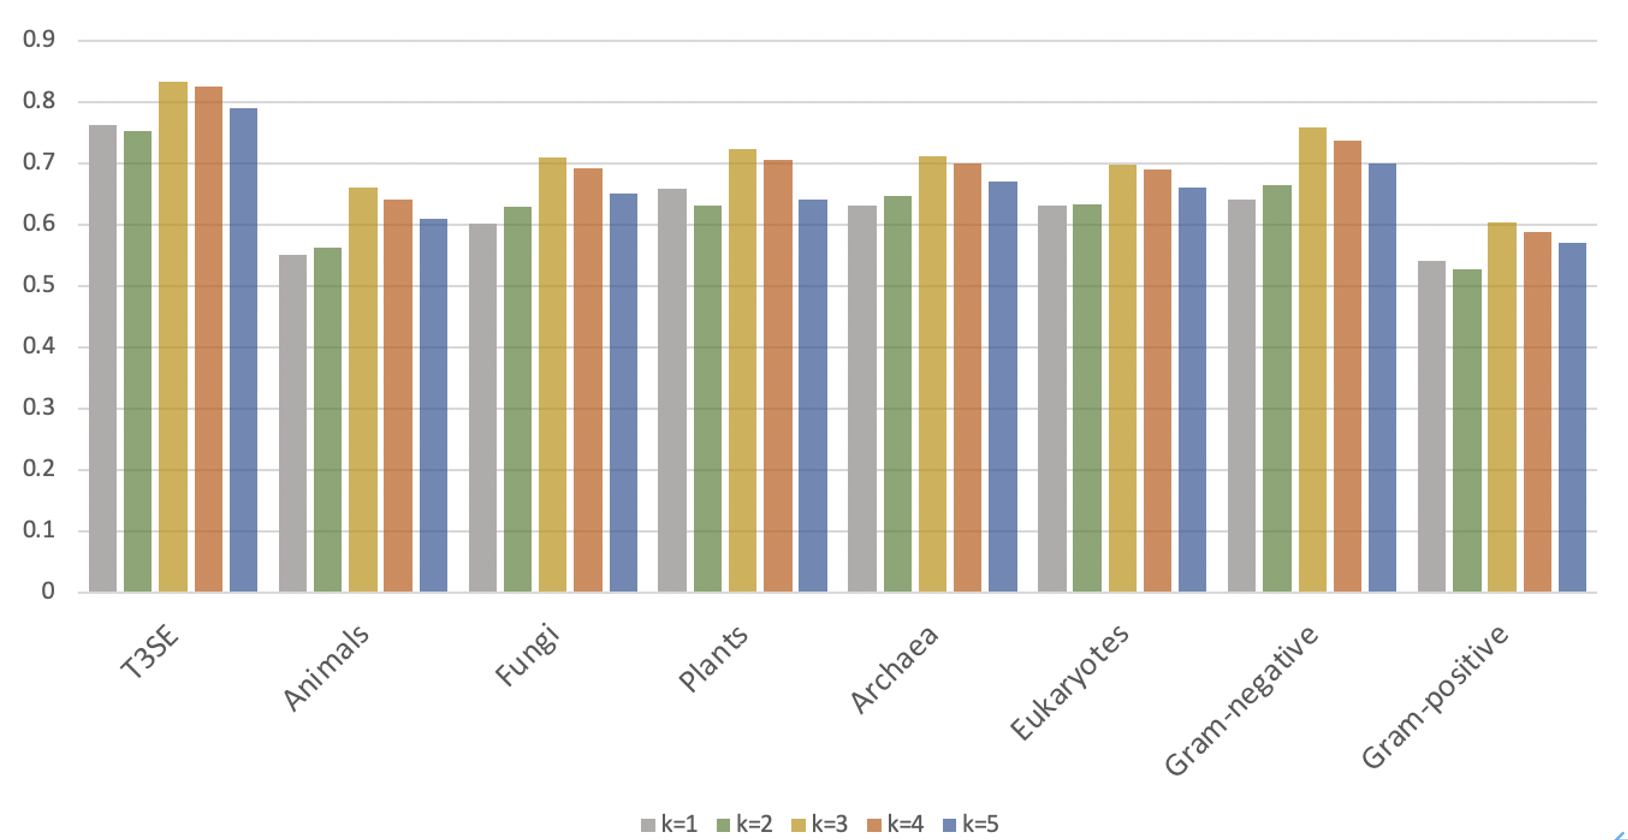
\includegraphics[width=1\textwidth]  {imgs/k-mer.png}
\bicaption[不同 k 值下 ProtPlat 模型的 $F_1$ 值比较]
        {不同 k 值下 ProtPlat 模型的 $F_1$ 值比较。}
        {Comparison of F1 scores obtained by ProtPlat with different values of k.}
\label{fig:k-mer}
\end{figure}


\section{ProtPlat web server}
我们将 ProtPlat 模型作为可供公众访问的网络服务 (https://compbio.sjtu.edu.cn/)。 Web server 的首页界面如图 \ref{fig:web-home} 所示。其中,Home Tab 是 ProtPlat web server的首页介绍,Upload Tab 是上传界面,如图 \ref{fig:web-upload}所示,用户可以按照界面上的要求上传任务的训练集和测试集。Web server upload 的背景模型是经过基于 Pfam 数据库的家族分类任务进行预训练的嵌入表征学习模型,可以用于进行蛋白质分类任务预测。用户可以将自己的训练集和测试集上传到服务器,系统将使用上传的训练集数据对预训练的 Prot Plat 模型进行微调,并在网页上就会显示测试数据集的预测结果。此外,用户还可以下载基于预训练的 ProtPlat 模型氨基酸嵌入向量(在下载选项卡中)。

由于在许多蛋白质分类问题中,训练集太小而无法支持从输入数据中学习好的蛋白质嵌入表征,在许多蛋白质分类问题共享从其氨基酸序列中提取的共同特征,小数据任务可以从两阶段训练策略(预训练 + 微调)中受益很多。


\begin{figure}[!htbp] 
\centering
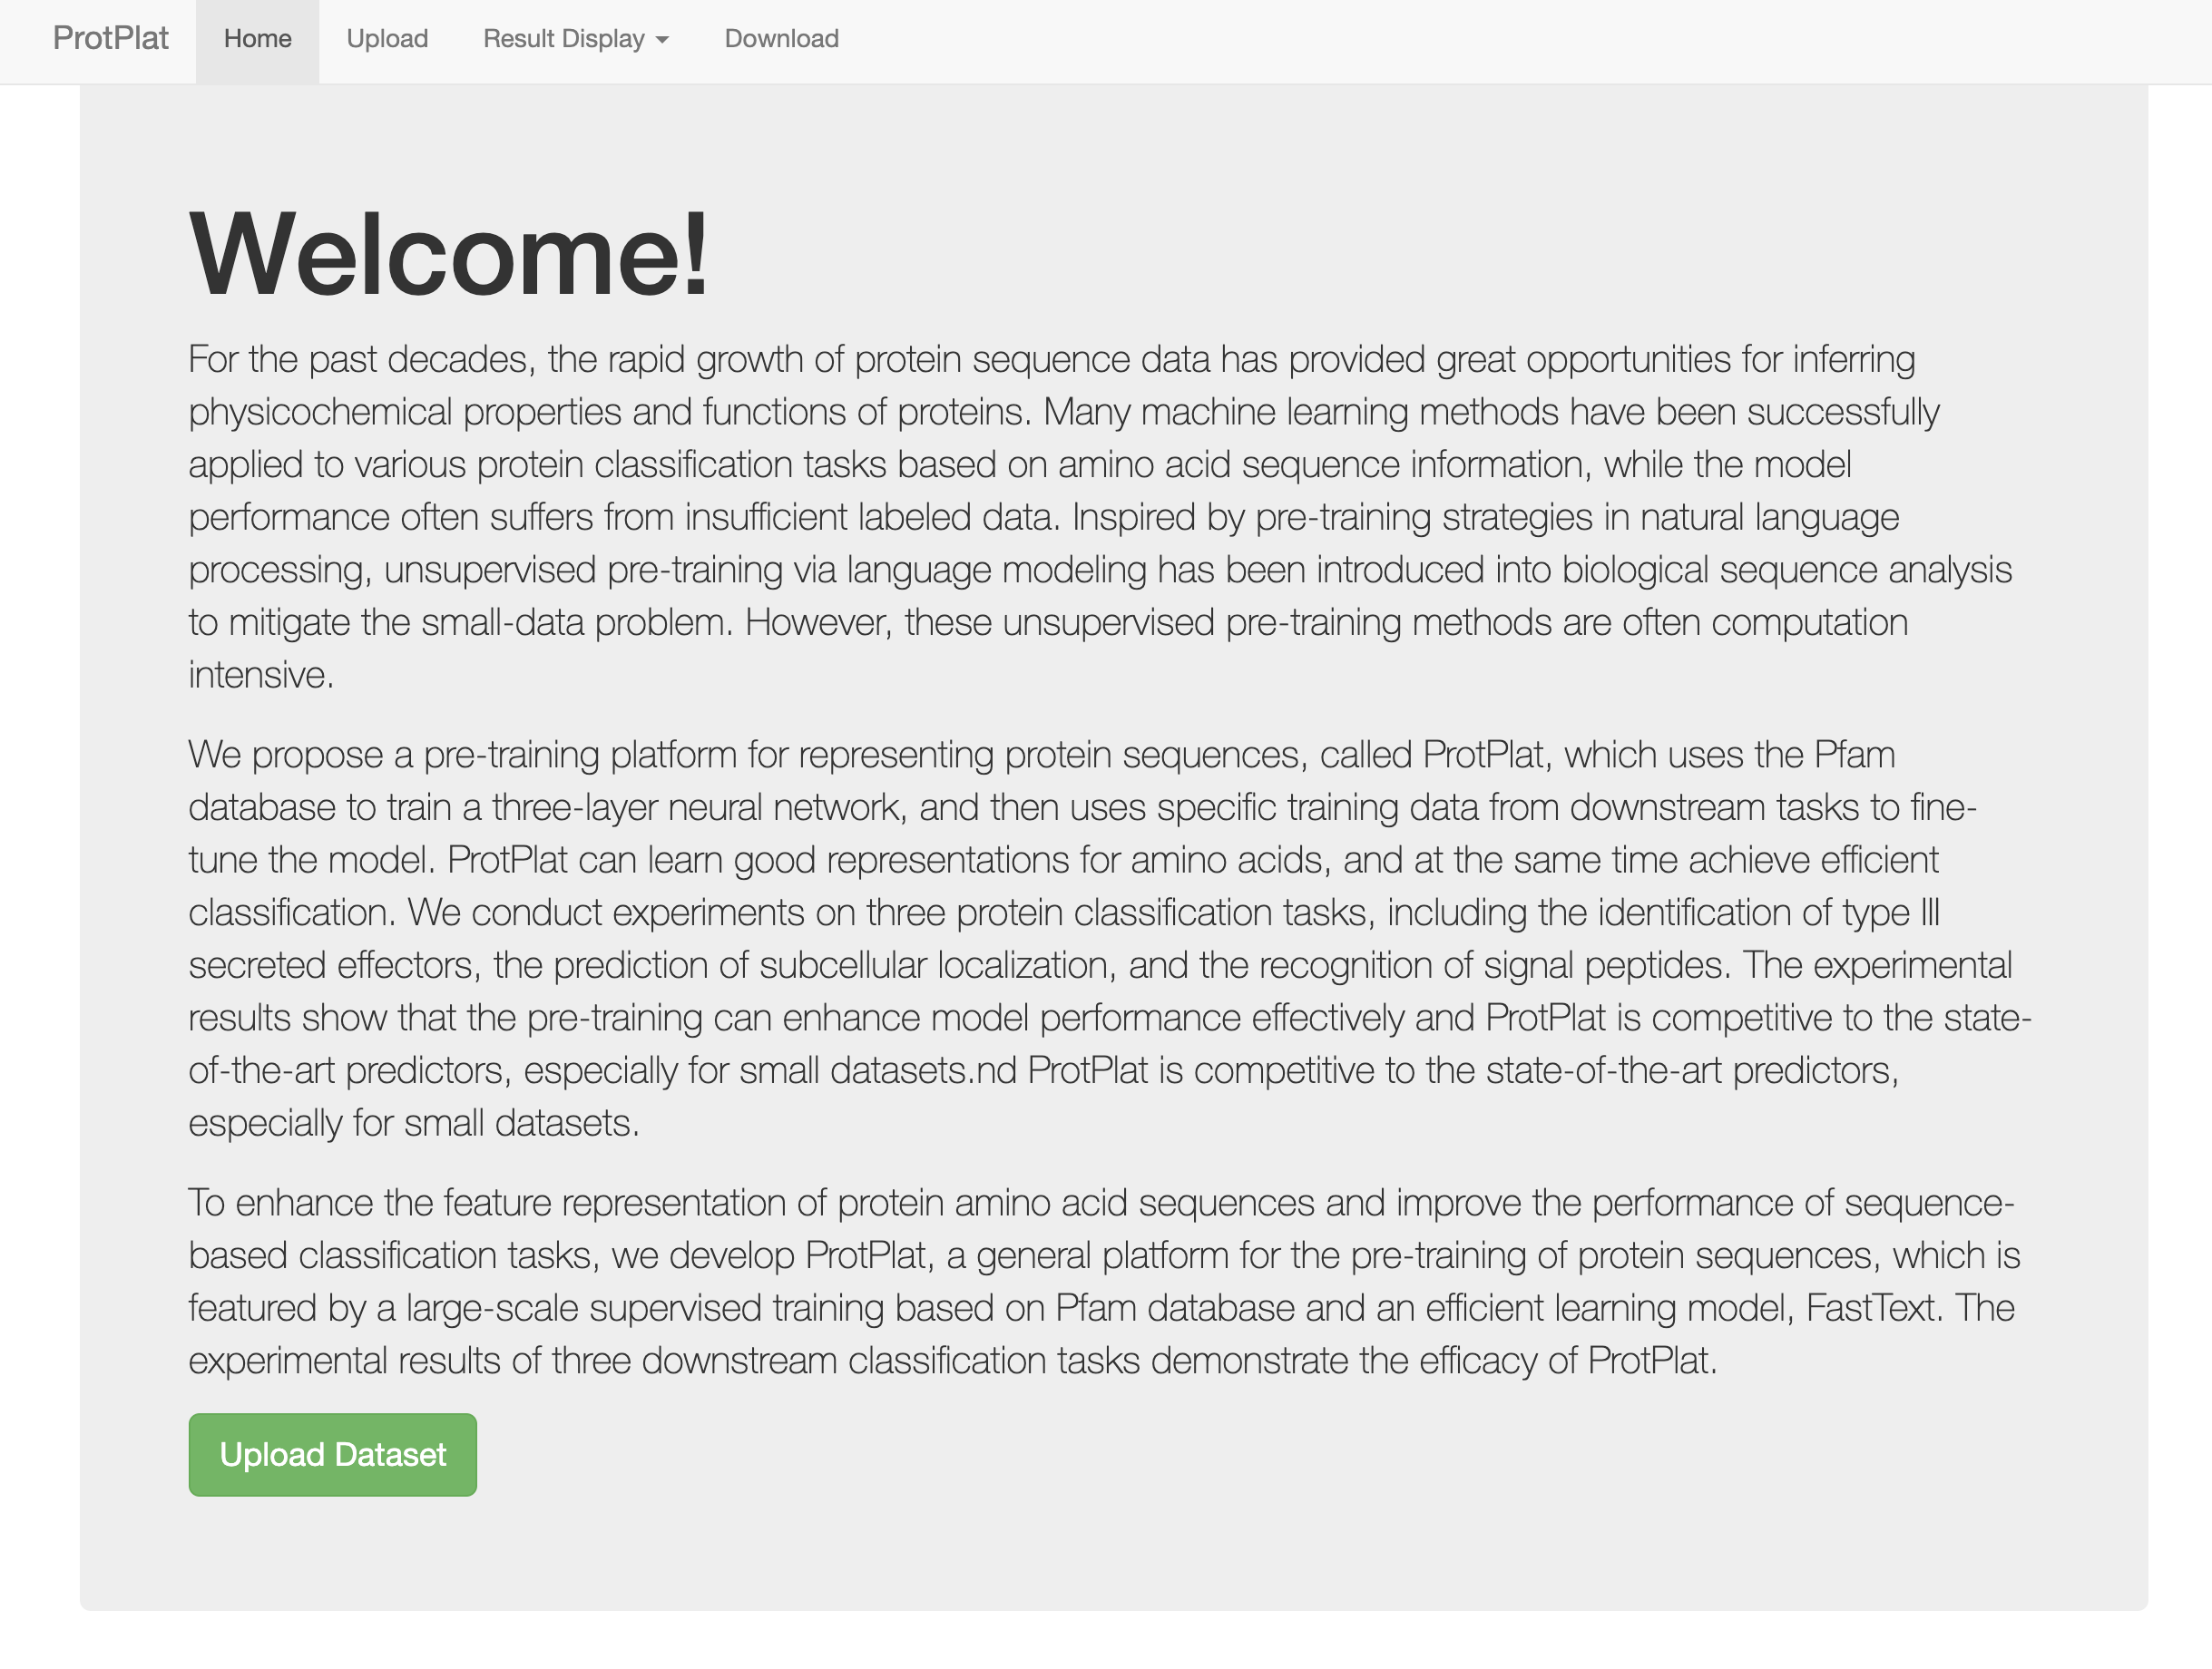
\includegraphics[width=0.8\textwidth]  {imgs/web-home.png}
\bicaption[ProtPlat 的 Web server 首页]
        {ProtPlat 的 Web server 首页。}
        {ProtPlat's web server homepage.}
\label{fig:web-home}
\end{figure}

\begin{figure}[!htp] 
\centering
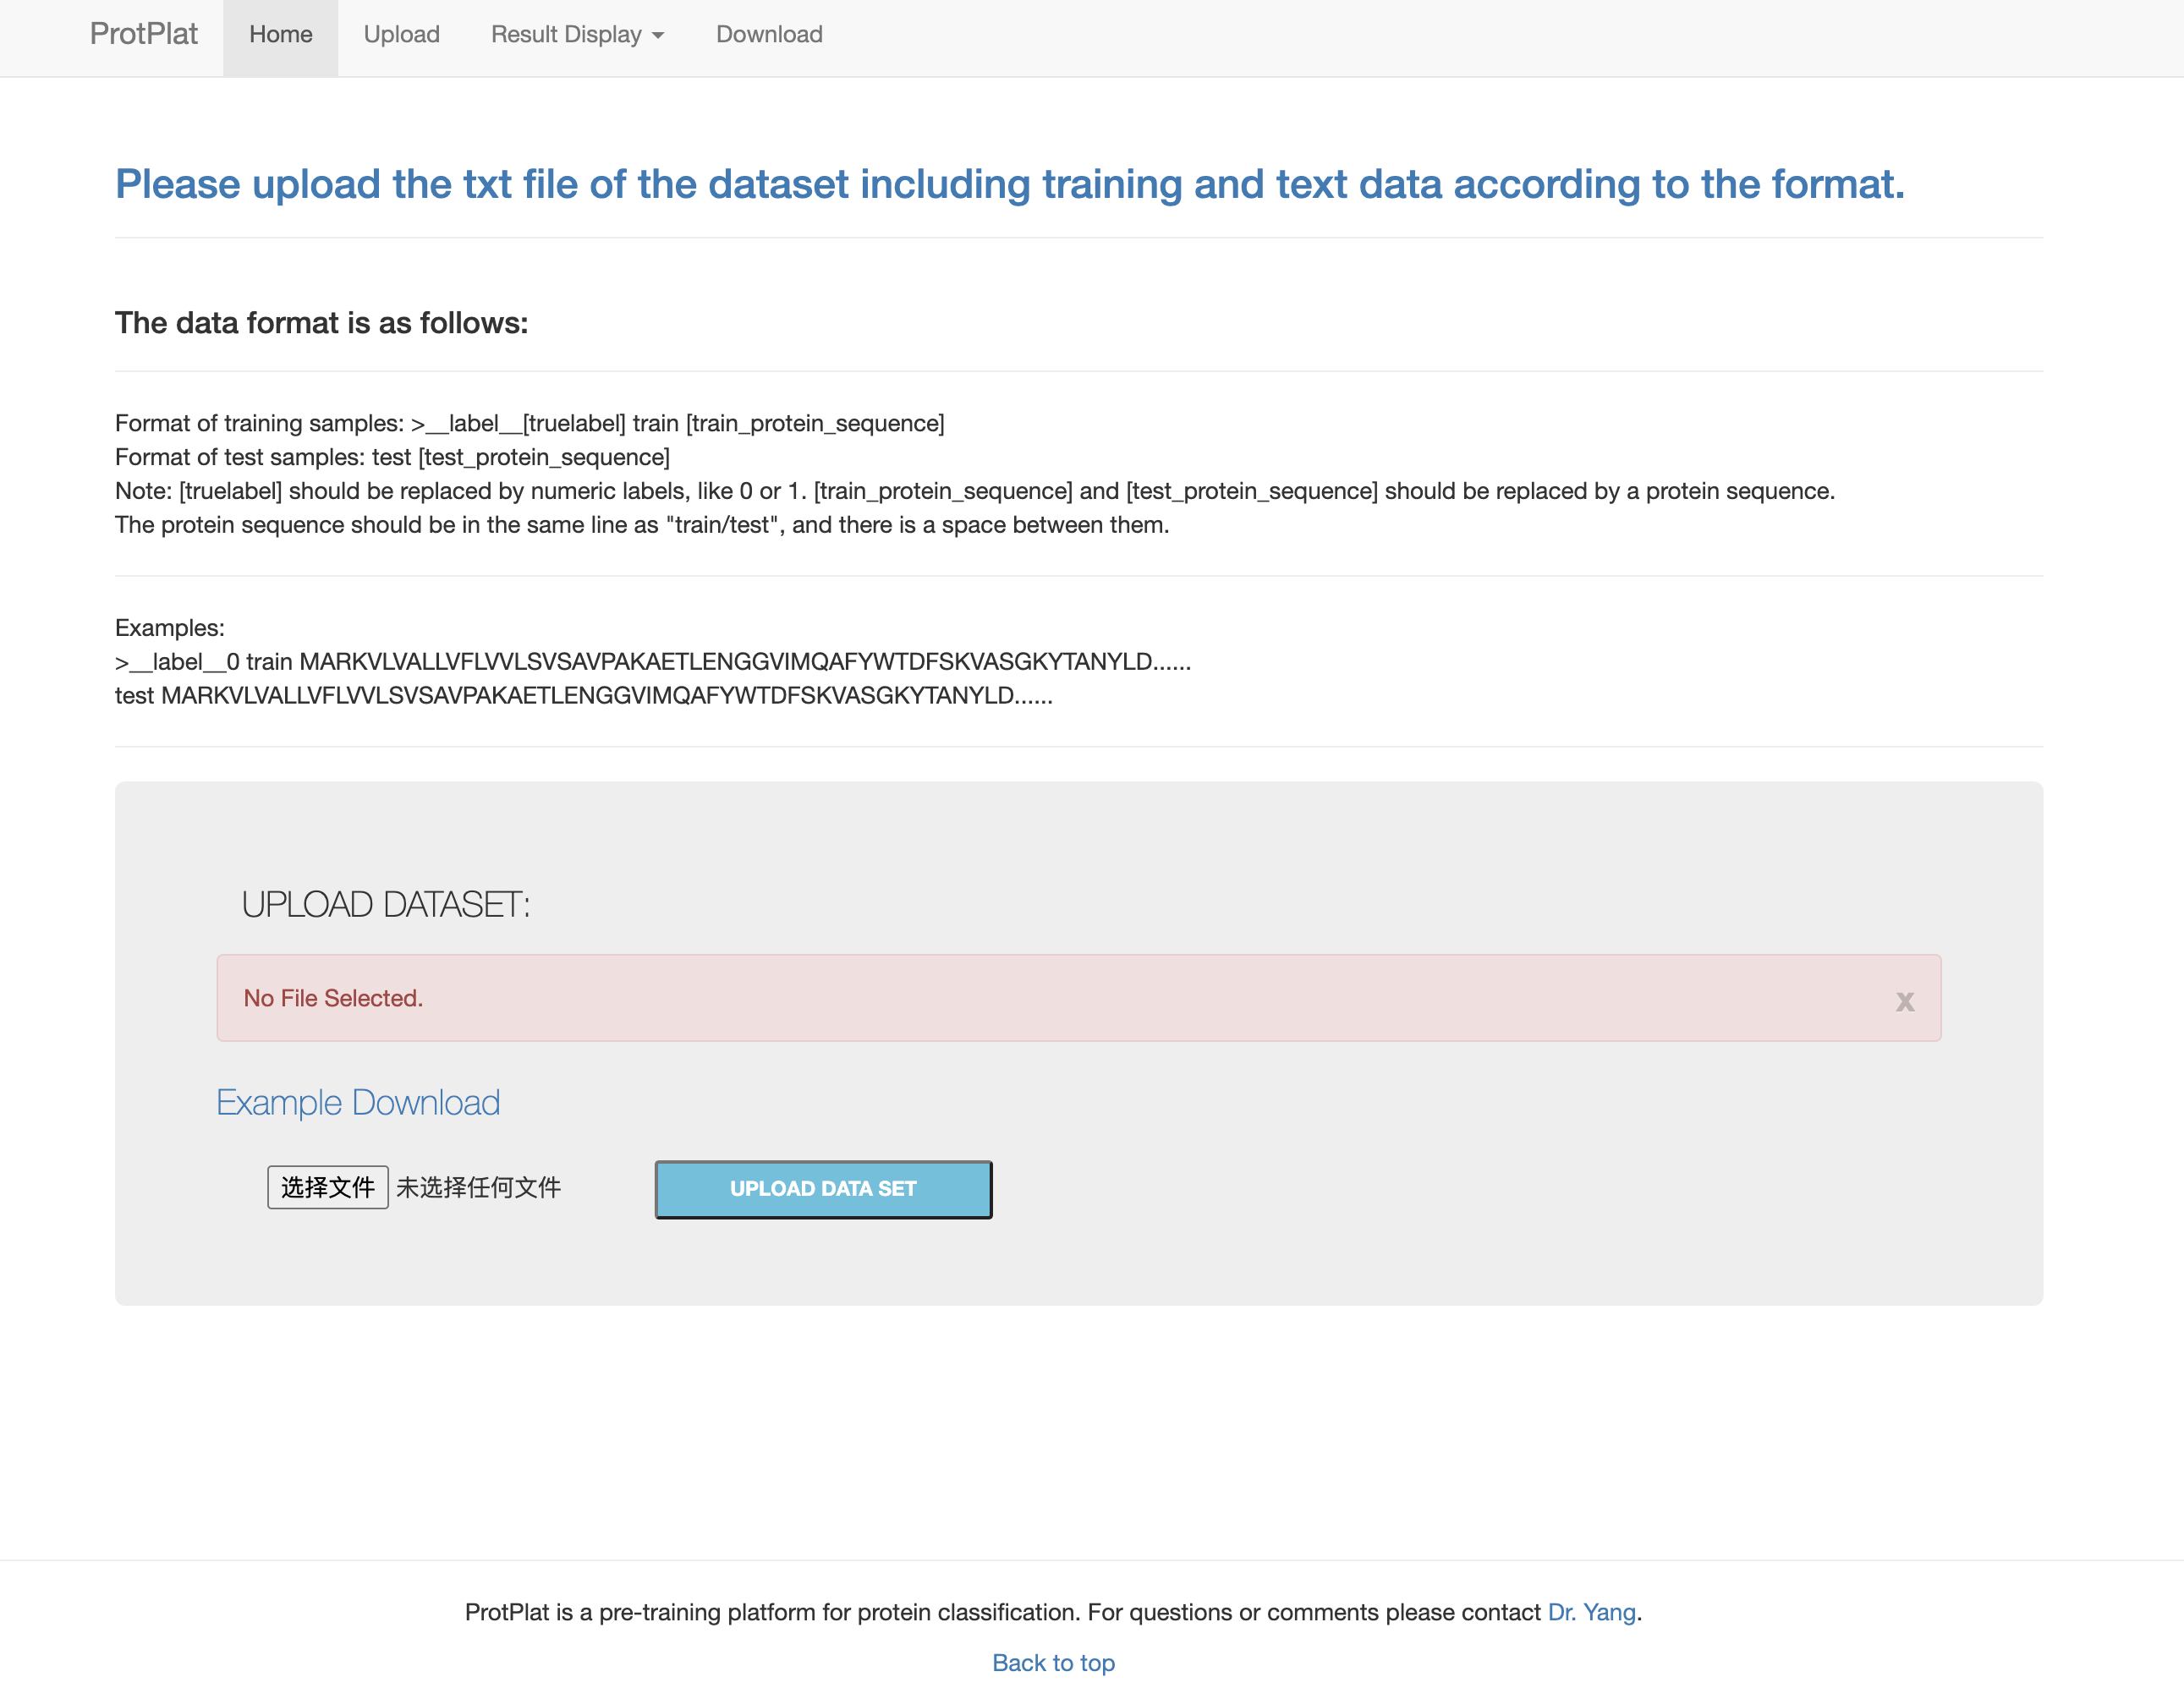
\includegraphics[width=0.8\textwidth]  {imgs/web-upload.png}
\bicaption[ProtPlat 的 Web server 首页]
        {ProtPlat 的 Web server 上传界面。}
        {ProtPlat's web server upload page.}
\label{fig:web-upload}
\end{figure}


\section{本章小结}
本章详细介绍了我们提出的基于有监督预训练得到的 ProtPlat 模型,可以在预训练阶段对大型数据库的蛋白质序列进行嵌入表征学习,在下游任务中对模型进行微调并解决蛋白质序列的分类问题。我们首先介绍了预训练和下游任务所需的实验数据集,接着从数据处理,模型介绍和实验结果三个方面详细介绍了 ProtPlat 模型基于预训练的蛋白质序列嵌入表征学习和基于微调的解决蛋白质序列分类任务两阶段过程。我们在下游的蛋白质序列分类任务中验证了嵌入表征学习具有良好的预测结果,并且通过消融实验验证了蛋白质序列划分的可行性和预训练过程中超参数选取的合理性。

\input{contents/math_and_citations}
\input{contents/floats}
\input{contents/summary}

%TC:ignore

% 参考文献
\printbibliography[heading=bibintoc]

% 附录
\appendix

% 附录中图表不加入索引
\captionsetup{list=no}

% 附录内容
\input{contents/app_maxwell_equations}
\input{contents/app_flow_chart}

% 结尾部分
\backmatter

% 用于盲审的论文需隐去致谢、发表论文、科研成果、简历

% 致谢
\input{contents/acknowledgements}

% 发表论文、科研成果
% 盲审论文中,发表论文及科研成果等仅以第几作者注明即可,不要出现作者或他人姓名
\input{contents/publications}
\input{contents/achievements}

% 简历
\input{contents/resume}

% 学士学位论文要求在最后有一个大摘要,单独编页码
\input{contents/digest}

%TC:endignore

\end{document}
